\documentclass[10pt]{article}
\usepackage{color}
\usepackage{bm}
% \usepackage{times}
\usepackage{amssymb, amsfonts, amsmath}
\usepackage{fancyhdr, fancyvrb}
\usepackage[framed, thmmarks]{ntheorem}
\usepackage{etoolbox}
\usepackage{bm, graphicx, graphics, url, natbib, paralist, afterpage, verbatim}
\usepackage{listings}
\usepackage{epstopdf}
\usepackage{bm, graphicx, graphics, url, natbib, paralist, afterpage, verbatim}
\usepackage{listings}
\usepackage{subfigure}
\usepackage{cleveref}
\usepackage[table,xcdraw]{xcolor}
\usepackage{rotating}



\newtheorem{proposition}{Proposition}
\newtheorem{definition}{Definition}
\newtheorem{remark}{Remark}
\newtheorem{corollary}{Corollary}
\newtheorem{result}{Result}
\newtheorem{theorem}{Theorem}
\newtheorem{lemma}{Lemma}

% \makeatletter

% \newcommand{\openbox}{\leavevmode
%   \hbox to.77778em{%
%  \hfil\vrule
%  \vbox to.675em{\hrule width.6em\vfil\hrule}%
%  \vrule\hfil}}
\makeatletter
\newcommand{\openbox}{\leavevmode
  \hbox to.77778em{%
  \hfil\vrule
  \vbox to.675em{\hrule width.6em\vfil\hrule}%
  \vrule\hfil}}
\gdef\proofSymbol{\openbox}
\newcommand{\proofname}{Proof.}
\newcounter{proof}\newcounter{currproofctr}\newcounter{endproofctr}%
\newenvironment{proof}[1][\proofname]{
  \th@nonumberplain
  \def\theorem@headerfont{\itshape}%
  \normalfont
  %\theoremsymbol{\ensuremath{_\blacksquare}}
  \@thm{proof}{proof}{#1}}%
  {\@endtheorem}
\makeatother


\bmdefine\mmu{\mu}


\setlength{\textheight}{9in} \setlength{\topmargin}{-0.5in}
\setlength{\textwidth}{6.0in} \setlength{\oddsidemargin}{+.13in}
\setlength{\evensidemargin}{-.1in}

\usepackage{xcolor}
\newcommand{\red}[1]{{\textcolor {red} {#1}}}


\title{Reconstruction of molecular network evolution from cross-sectional omics data}
\author{ {\small
\textbf{Mehran Aflakparast}$^{1}$, \textbf{Mathisca C.A. de Gunst}$^{1}$,\textbf{Wessel N. van Wieringen}$^{1,2,}$%\footnote{Corresponding author. Email: w.vanwieringen@vumc.nl}
}
\\
{\small $^1$ Department of Mathematics, VU University Amsterdam}
\\
{\small De Boelelaan 1081a, 1081 HV Amsterdam, The Netherlands}
\\
{\small $^2$ Department of Epidemiology and Biostatistics, VU University Medical Center}
\\
{\small P.O. Box 7057, 1007 MB Amsterdam, The Netherlands}
}
\date{}



\makeatletter
\newcommand*{\rom}[1]{\expandafter\@slowromancap\romannumeral #1@}
\makeatother

\begin{document}
\maketitle


\begin{abstract}
\noindent
Cross-sectional studies may shed light on the evolution of a disease like cancer through the comparison of patient traits among disease stages. 
This problem is especially challenging when a complex trait like a gene-gene interaction network reconstructed from omics data is considered, and, in addition, the patients of each stage need not form a homogeneous group. Here the problem is operationalized as the estimation of stage-wise mixtures of Gaussian graphical models (GGMs) from high-dimensional data. These mixture are fitted by a (fused) ridge penalized EM algorithm. The fused ridge shrinks GGMs of contiguous stages. The ridge penalty parameters are chosen through cross-validation. The proposed estimation procedures are shown to be consistent and their performance in other respects is studied in simulation. The down-stream exploitation of the fitted GGMs is outlined. In a data illustration the methodology is employed identify gene-gene interaction network changes in the transition from normal to cancer prostate tissue.
\\
\\
{\bf Keywords:}  Conditional (in)dependence; Fused ridge; Gaussian graphical model; $\ell_2$-penalization; Mixture model; Multivariate normality;
\end{abstract}

% The precision matrix harbours the relations among the variates: a zero off-diagonal element corresponds to the two corresponding variates being conditionally independent on all other variates, whereas non-zero indicate conditional dependence. The relations among the variates may differ between stage and subgroup. These changes shed light on the evolution of the regulatory architecture of the variates during the course of the disease.


% Within each subgroup$\times$stage-combination the relations among the $p$ variates measured are described by a Gaussian graphical model. Hence, $\mathbf{Y}_{\ast, i} | i \in v_{t, k_t} \sim \mathcal{N}(\mmu_{t, k_t}, \mathbf{\Omega}_{t, k_t}^{-1})$.

\section{Introduction}
Cancer is not a one but a collection of multiple diseases \textbf{(REF)}. It is heterogeneous within a tumor, between tissues, and between individuals. This heterogeneity can be witnessed in the many oncogenomics studies that uncover novel clinically meaningful subgroups in cancer of a particular tissue from transcriptomic data \textbf{(REFS)}. The origin of this heterogeneity is found in the evolutionary nature of the cancer \textbf{(REF)}. Simplistically, cancer is initiated by abnormalities at the molecular level of the cell that result in dysregulation of its gene-gene interaction network. When these abnormalities (through its dysregulatory consequences) increase the fitness of the proginetor cancer cells they are passed on to daughter cells. The daughter cells accumulate further and varying abnormalities leading to more dysregulation. Consequenty, the collection of cells that form a tumor harbour many different molecular abnormalities and dysregulatory patterns. Here we aim to uncover the dysregulatory changes of the gene-gene interaction network over time through the analysis of cross-sectional omics studies.

A cross-sectional study is a clinical study with a particular set up \textbf{(REF TO DESIGN BOOK)}. All patients included have the same disease. However, they originate from different stages of the disease. For instance, prostrate cancer is believed to develop from normal tissue via pre-cursor lesions to cancer after which it metastasizes \textbf{(REF)}. As such the included patients represent the course of the disease. Hence, comparison of the (traits of) patients from contiguous stages provides information on the evolution of the disease.

The cellular regulatory system is described by a network. A network comprises of nodes and edges. Nodes represent the genes while edges correspond to the relations among the genes. Here these relations are operationalized by conditional independencies. An edge between two genes is absent/present if this gene pair is conditional independent/dependent given all other genes.

Transcriptomic data obeying a network is often described by a Gaussian graphical model (GGM). A GGM assumes the data are multivariate normally  distributed with a particular parametrization of the inverse of the covariance matrix (the precision matrix). Whenever an edge between two genes is absent in the network, the element of the precision matrix corresponding to the gene pair exhibits a zero. A zero in the precision matrix ensures the multivariate normal density factorizes with respect to the two genes, implying their conditional independence given all other network nodes.

In practice knowledge of the regulatory network is often unavailable or partially known at best. The network can be reconstructed from data through the estimation of the precision matrix and the study of its support. The estimation of a GGM is frustrated by the high-dimensionality of the data which is overcome by invoking penalization. Typically, GGMs are estimated through the maximization of the log-likelihood in subject to either a lasso or ridge penalty that constraints the sum of the size of the precision elements \textbf{(REF TO FRIEDMAN AND VAN WIERINGEN)}. When the data stem from groups and a separate GGM needs to be estimated per group, these `traditional' penalties are augmented with a fused component. This augmentation penalizes the difference between precision matrices from different groups (see \citet{Bilg2015,danaher2014joint,guo2011joint,zhu2014structural}). 

The heterogeneity of the disease is reflected in patients from the same disease stage forming a multitude of subgroups. Gene-gene interaction networks may then differ among subgroups and need to be reconstructed per subgroup. As subgroups are unknown this amounts to learning a mixture of GGMs. 
Several methods for the estimation of GGM mixtures from high-dimensional data have been put forward 
(see for example~\citet{raftery2006variable,maugis2009,maugis2011non,ruan2011,lotsi2013,hill2013,azizyan2015}). However, none of these methods address the cross-sectional design where the data originates from multiple disease stages.


Here we consider the problem of learning the evolution of a gene-gene interaction network (operationalized as GGM) from cross-sectional, high-dimensional data in the face of heterogeneity. This is addressed through fused ridge penalized estimation of a (combination of) mixture(s) of GGMs. The paper is organized as follows. We first introduce the concept of an disease graph that specifies the evolutionary relations among the disease subgroups over the stages. At each disease stage the subgroup information is unknown and its data are described by a mixture of Gaussian graphical models describing the conditional independence network among genes within each mixture component. Subsequently, two methods for the model estimation are presented. One methods constructs the disease graph sequentially whereas the other assumes it known but afterwards selects the best disease graph. Both methods employ a penalized EM algorithm but with a different penalty structure to incorporate the assumed disease graph knowledge. The consistency of these estimators is shown next. The next section provides methodology to sparsify the resultant subgroup networks and introduces network measures to identify topological changes between the disease stages. The methodology is evaluated in a small scale simulation. Finally, the developed methodology is illustrated on transcriptomic data on the Notch signalling pathway from six multi-stage prostate cancer studies.





\section{Experimental design, data and model}\label{sec:design}
Consider a cross-sectional clinical study. The study comprises $n$ independent samples obtained from $T$ subsequent stages of a disease. Each sample belongs to a single, known disease stage (although the method assigning samples to stages may be error-prone). The severity of the disease stage increases with $t$, $t=1, \ldots, T$. Stage $t$ includes $n_t$ samples. Then, $n = \sum_{t=1}^T n_t$.

Of each sample the same $p$ characteristics have been measured. The $p$-variate random variable $\mathbf{Y}_{\ast, i}$ (or, when permitted by the context denoted simpler as $\mathbf{Y}_i$) represents the measurements of the $p$ characteristics of sample $i$ for $i=1, \ldots, n$. Together these $n$ data vectors constitute the data matrix $\mathbf{Y}_{\ast, \ast}$ (or, simpler $\mathbf{Y}$), with columns containing the $\mathbf{Y}_{\ast, i}$. Augmented with the design, $\mathbf{Y}$ comprises the full information from the study.

Before the model is presented, the relations among the disease stages need specification. The descendancy of these stages is assumed to follow a (temporarily) known tree structure given by the `disease graph' $\mathcal{G}^s = (\mathcal{V}^s, \mathcal{E}^s)$, where superscript $s$ refers to the graph relating the subgroups of the disease stages. Let $v_{1,1}^s$ be the root node representing the first stage (e.g. the healthy control). All samples $i$ such that $i = 1, \ldots, n_1$ belong to this stage. The root node stage may give birth to (say) $K_2$ subgroups at the next (second) stage. And so on. In general, let nodes $v_{t,1}^s, \ldots, v_{t, K_t}^s$ represent the various ($K_t$) subgroups co-existing at disease stage $t$. Then, $pa(v_{t, k_t}^s) \in \{ v_{t-1, 1}^s, \ldots, v_{t-1, K_{t-1}}^s \}$ for all $k_t = 1, \ldots, K_t$. An illustration of the evolution of the disease subgroups is provided in Figure \ref{fig.diseaseEvolution}.

\begin{figure}[h!]
\begin{center}
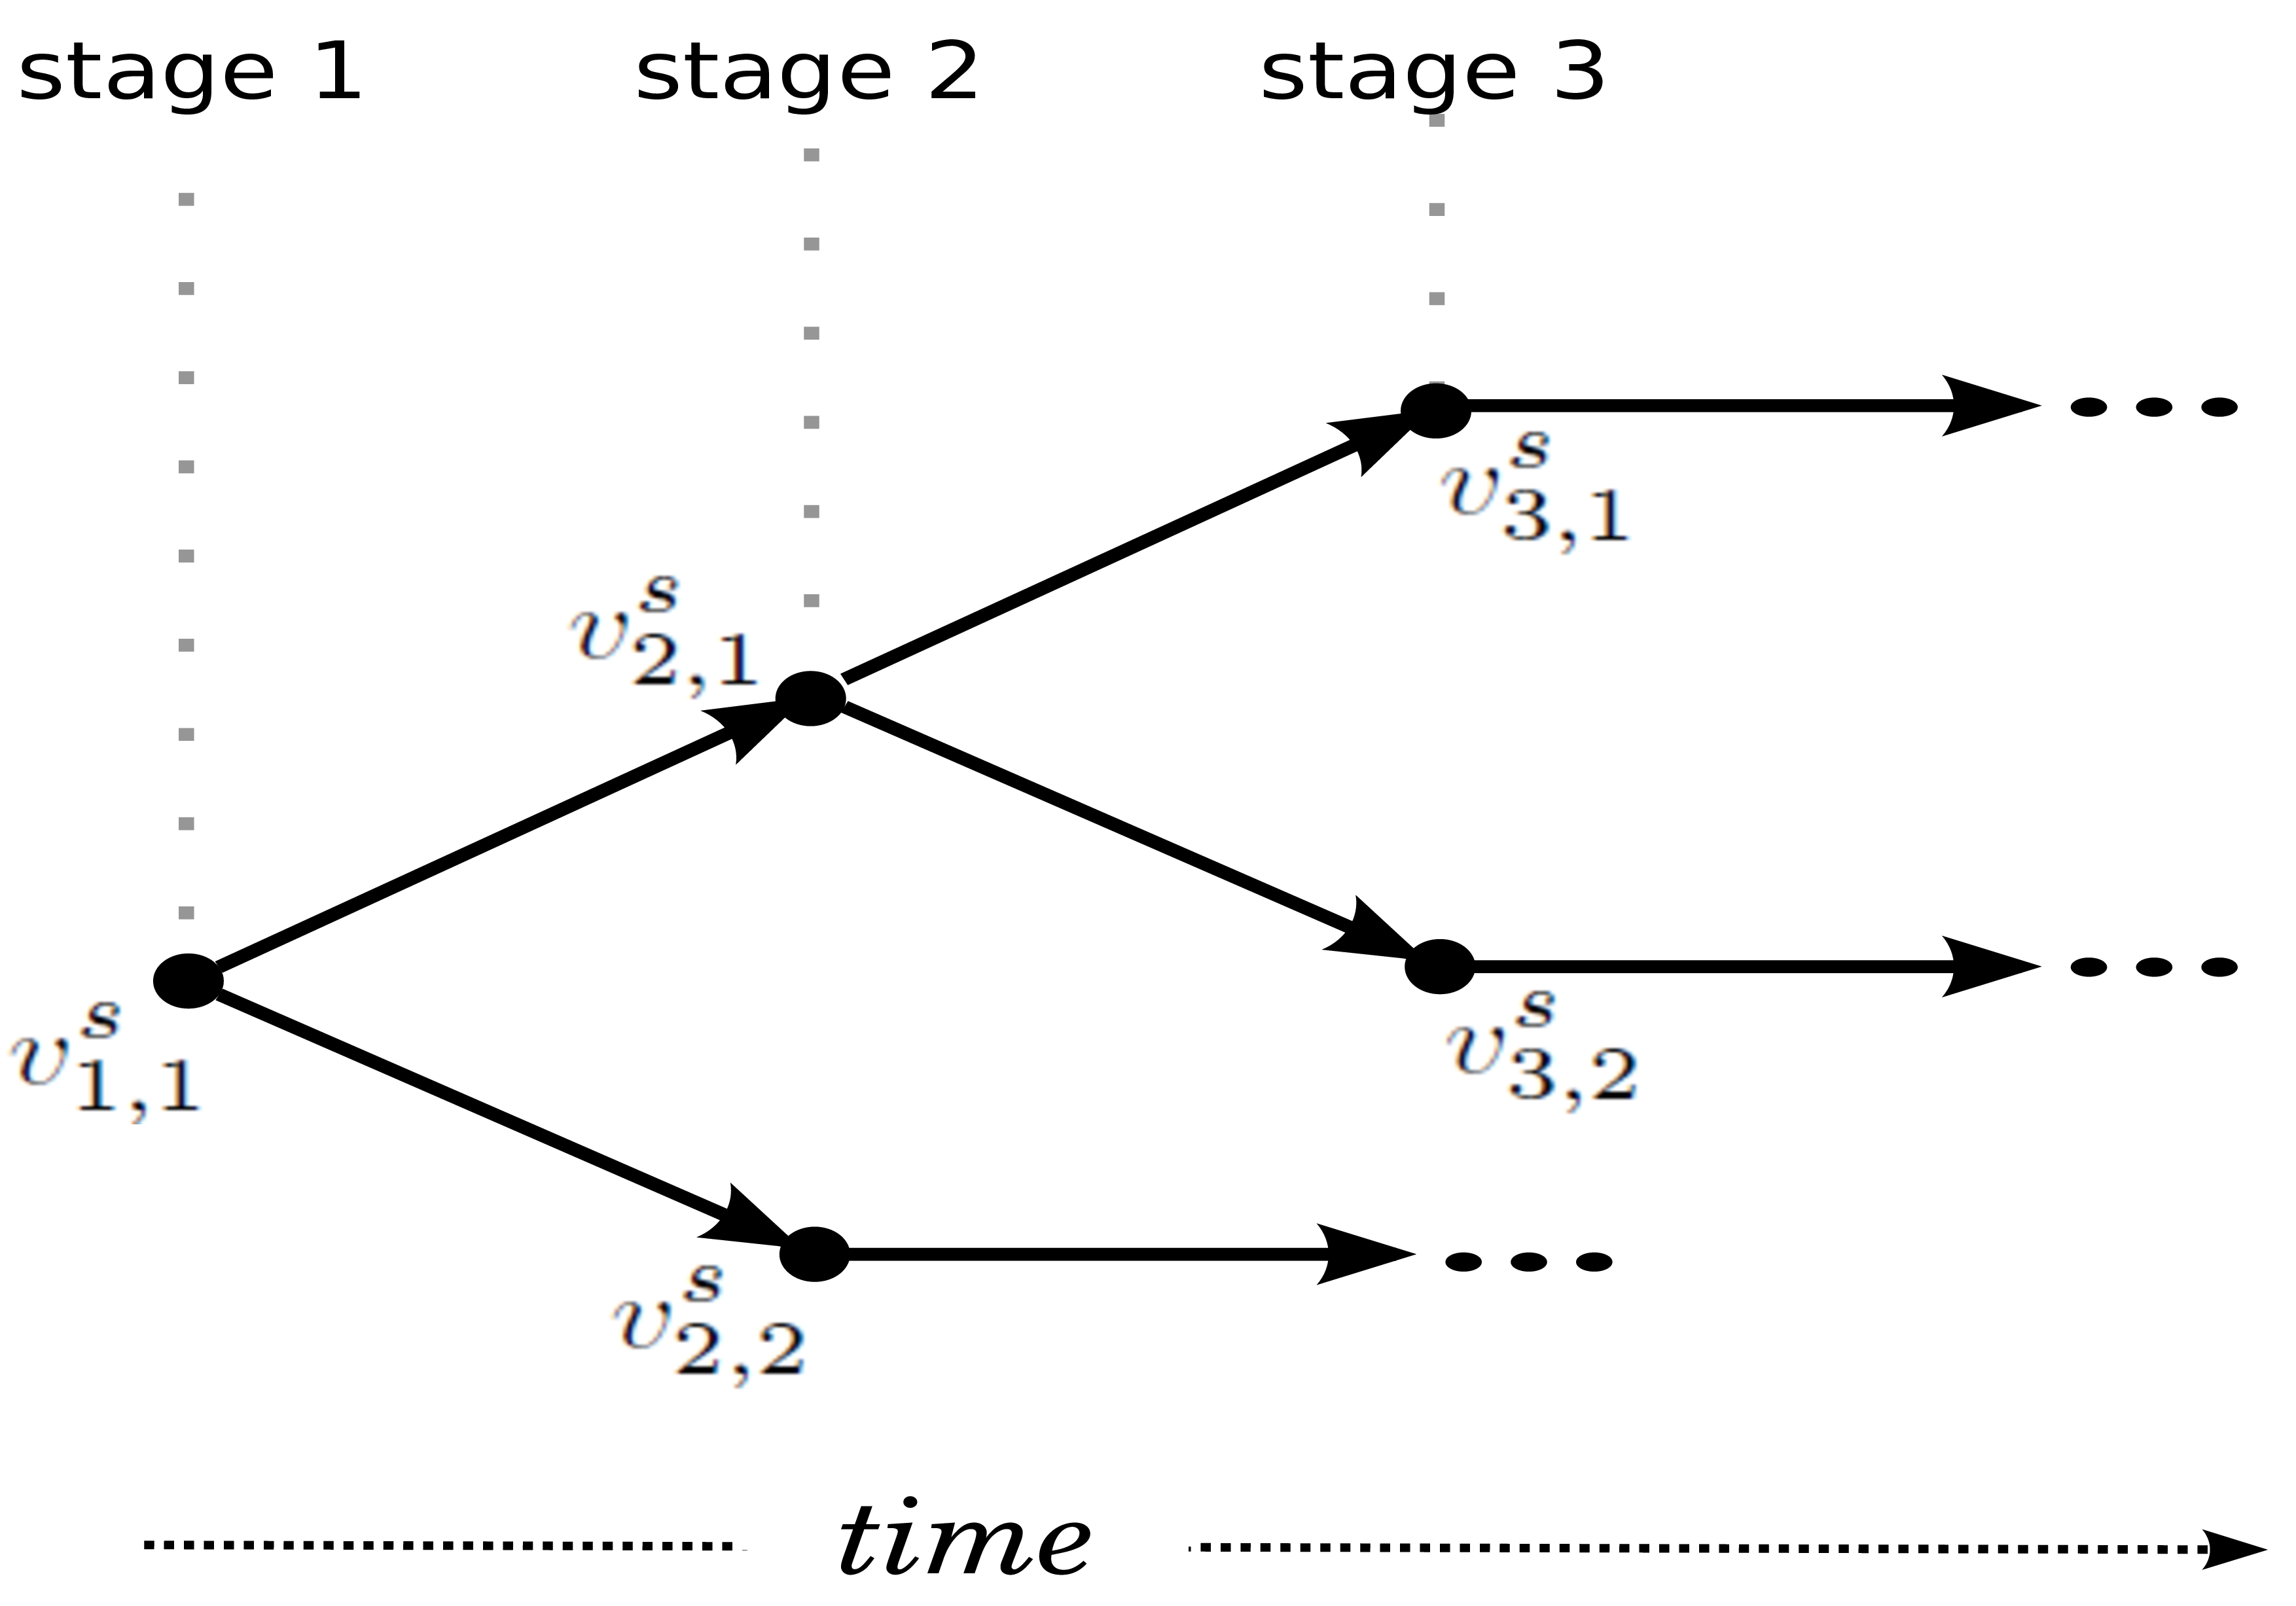
\includegraphics[angle=0, scale=0.07]{stages2subgroups.png}
\end{center}
\caption{Evolution of the subgroups of a disease.}
\label{fig.diseaseEvolution}
\end{figure}


With the subgroup information generally being unavailable, the random variable $\mathbf{Y}_i$ is assumed to follow a mixture model. The mixture components, corresponding to a
subgroup$\times$stage-combination, are multivariate Gaussians: $\mathbf{Y}_{i} \, | \, i \in v_{t, k_t}^s \sim \mathcal{N}(\mmu_{v_{t, k_t}^s}, \mathbf{\Omega}_{v_{t, k_t}^s}^{-1})$. Convolution with a discrete mixing distribution yields:
\begin{eqnarray} \label{form:mixtureModel}
\mathbf{Y}_{i} & \sim & \sum_{k_t=1}^{K_t} \pi_{v_{t, k_t}^s} \mathcal{N}(\mmu_{v_{t, k_t}^s}, \mathbf{\Omega}_{v_{t, k_t}^s}^{-1}) \qquad \mbox{for } i=1, \ldots, n,
\end{eqnarray}
with $\pi_{v_{t, k_t}^s} = P(i \in v_{t, k_t}^s )$ the mixing proportions. As the precision matrices $\{ \mathbf{\Omega}_{v_{t, k_t}^s} \}$ harbor the relations among the variates at each stage, differences between precision matrices of different stages and subgroups shed light on the evolution of the regulatory architecture among the variates over the course of the disease.


% with $\pi_{v_{t, k_t}^s} = P(i \in v_{t, k_t}^s )$ the mixing proportions. To capture the evolutionary relations among  descendant subgroups their precision matrices are modeled through $\mathbf{\Omega}_{v_{t, k_t}^s} = \mathbf{\Omega}_{pa(v_{t, k_t}^s)}  + \mathbf{\Theta}_{v_{t, k_t}^s}$ for all $t$ with $\mathbf{\Theta}_{v_{t, k_t}^s}$ a $p \times p$ symmetric matrix such that $\mathbf{\Omega}_{pa(v_{t, k_t}^s)}  + \mathbf{\Theta}_{v_{t, k_t}^s} \succ 0$. The precision of subgroup $v_{t, k_t}^s$ is thus a perturbation of that of its parent subgroup. As the precision matrices $\{ \mathbf{\Omega}_{v_{t, k_t}^s} \}$ harbor the relations among the variates at each stage, differences (parameterized by the $\mathbf{\Theta}_{v_{t, k_t}^s}$) between precision matrices of different stages and subgroups shed light on the evolution of the regulatory architecture among the variates over the course of the disease.


\section{Estimation}
The parameters of the presented mixture model are estimated by ridge penalized maximum likelihood (ML). The log-likelihood equals:
\begin{eqnarray} \label{form:mixtureLikelihood}
\mathcal{L}(\mathbf{Y}; \mathbf{\Xi}) & \propto & \sum_{t=1}^T \sum_{i=n_{<t} + 1}^{n_{<t} + n_t} \log \Big[ \sum_{k_t=1}^{K_t}  \pi_{v_{t, k_t}^s} \phi_{\mmu_{v_{t, k_t}^s}, \mathbf{\Omega}_{v_{t, k_t}^s}^{-1}} (\mathbf{Y}_i) \Big],
\end{eqnarray}
where $n_{<t} = n_1 + \ldots + n_{t-1}$ and $\mathbf{\Xi} = \{ \{ \pi \}, \{ \mmu \}, \{ \mathbf{\Omega} \} \}$, the set of all model parameters. Below we present two estimation procedures. The first, stage-wise procedure considers the estimation of one stage at the time assuming all parameters of the preceding stage known. Initiated by the estimation of the first stage and running through the stages to the last yields estimates of all parameters. At each stage the number of subgroups needs to be determined. As such, this procedure reconstructs the disease graph on the fly. This is contrasted by a second procedure which estimates model (\ref{form:mixtureModel}) for a given disease graph (but subgroup information of the individuals still unknown). To account for the uncertainty in the disease graph, the latter procedure is augmented with a selection step which identifies the best (in some sense) disease graph from the set of all possible disease graphs.

% The last procedure is most general and estimates all model parameters simultaneously. The first two procedures are illustrative for the last, but of interest in their own right.


\subsection{Stage-wise reconstruction}\label{sec:stagewise}
Stage-wise reconstruction of the disease graph amounts to the estimation of Model (\ref{form:mixtureModel}) for samples from stage $t$ while parameters of previous stages are assumed known. Model (\ref{form:mixtureModel}) is estimated by a penalized EM (Expectation-Maximization) algorithm. For the presentation this algorithm, we introduce the latent variable $Z_{i, k_t} = I_{\{ i \in v_{t,k_{t}}^s \}} \in \{ 0, 1\}$ indicating the sample $i$'s subgroup of the disease graph. The E-step then amounts to the estimation of these $Z_{i,k_t}$ (by their expectation), given the current (penalized) estimates of the parameters of model (\ref{form:mixtureModel}). With estimates of the $Z_{i,k_t}$ at hand, the M-step re-estimate the model parameters by ridge penalized maximum likelihood. These steps are applied iteratively, until convergence.
\\
\vspace{-5pt}
\\
\textbf{E-step}
\\
The derivation of the expectation of the latent variables $Z_{i, k_t}$ is unchanged by the employed penalization of the log-likelihood (and we thus refer to \citet{Titt1985}). Hence, given an estimate of model parameters (aggregated in $\widehat{\mathbf{\Xi}}$) and the data, Bayes' theorem yields:
\begin{eqnarray*}
\hat{Z}_{i, k_t} = E( Z_{i, k_t} \, | \, \mathbf{Y}; \widehat{\mathbf{\Xi}} ) = P(I_{\{ i \in v_{t,k_{t}}^s \}} = 1 \, | \, \mathbf{Y}; \widehat{\mathbf{\Xi}}) =
\frac{\hat{\pi}_{v_{t, k_t}^s} \phi_{\hat{\mmu}_{v_{t, k_t}^s}, \widehat{\mathbf{\Omega}}_{v_{t, k_t}^s}^{-1}} ( \mathbf{Y}_i = \mathbf{y}_i )}{
\sum_{k_t=1}^{K_t}  \hat{\pi}_{v_{t, k_t}^s} \phi_{\hat{\mmu}_{v_{t, k_t}^s}, \widehat{\mathbf{\Omega}}_{v_{t, k_t}^s}^{-1}} ( \mathbf{Y}_i = \mathbf{y}_i )}.
\end{eqnarray*}
A numericaly stable evaluation of this expression can be achieved as in the steps below: \textit{i)} calculate the individual's contributions (denoted $A_{i,k_t}$) on the log-scale $A_{i,k_t} = \log(\pi_k) - \tfrac{1}{2} p  \log(2\pi) + \log(|\mathbf{\Omega}_{k_t}|) - (\mathbf{Y}_i-\mmu_{k_t})^{\top}\mathbf{\Omega}_{k_t} (\mathbf{Y}_i-\mmu_{k_t})$, \textit{ii)} define $B_{i,k_t} = A_{i,k_t} - \max_{k_t} A_{i,k_t}$, then \textit{iii)} calculate $\hat{Z}_{i, k_t}$ through $\exp(B_{i,k_t}) / [ \sum_{k_t=1}^{K_t} \exp(B_{i,k_t}) ]$.
\\
\\
\textbf{M-step}
\\
Estimation of the parameters of model (\ref{form:mixtureModel}) under the assumption of the latent variables $Z_{i, k_t}$ known amounts to the maximization of the logarithm of the so-called complete likelihood:
\begin{eqnarray*}
\log \Big\{
\prod_{i=n_{<t}+1}^{n_t + 1} \prod_{k_t = 1}^{K_t} \big[ \pi_{v_{t, k_t}^s} \phi_{\mmu_{v_{t, k_t}^s}, \mathbf{\Omega}_{v_{t, k_t}^s}^{-1}} ( \mathbf{Y}_i = \mathbf{y}_i ) \big]^{Z_{i, k_t}} \Big\}.
\end{eqnarray*}
To cope with the high-dimensionality of the data, the complete log-likelihood is augmented with the ridge penalty \citep{VWie2014b}:
\begin{eqnarray*}
\lambda_2 \sum_{k_t=1}^{K_t}  \| \mathbf{\Omega}_{v^s_{t, k_t}} - \mathbf{T} \|_2^2 & = &  \lambda_2 \sum_{k_t=1}^{K_t} \mbox{tr} [ (\mathbf{\Omega}_{v_{t, k_t}^s} - \mathbf{T})^{\top} (\mathbf{\Omega}_{v_{t, k_t}^s} - \mathbf{T})].
\end{eqnarray*}
in which $\lambda_2$ is the ridge penalty parameter and $\mathbf{T} \succ 0$ is a symmetric, positive definite target matrix towards which the precision estimate of each subgroup is shrunken when $\lambda_2 \rightarrow \infty$. Then, after substitution of the $Z_{i, k_t}$  by their estimates obtained in the E-step, parameter estimates are updated by maximization of the penalized logarithm of the complete likelihood.

The maximization of the penalized log-likelihood with respect to parameters $\{ \pi \}$ and $\{ \mmu \}$, which are not involved in the ridge penalty, is fully analogous to the unpenalized case. Hence, they are estimated by:
\begin{eqnarray*}
\hat{\pi}_{v_{t, k_t}^s} = \frac{1}{n_t} \sum_{i=n_{<t}+1}^{n_{<t}+n_t} \hat{Z}_{i, k_t}  \qquad \mbox{ and } \qquad \hat{\mmu}_{v_{t, k_t}^s} = \Big( \sum_{i=n_{<t}+1}^{n_{<t}+n_t} \hat{Z}_{i, k_t} \mathbf{Y}_i \Big)  \Big/  \Big( \sum_{i=n_{<t}+1}^{n_{<t}+n_t} \hat{Z}_{i,k_t} \Big),
\end{eqnarray*}
in which the sums run only of the those samples belonging to stage $t$.

For the estimation of the subgroup's precision matrices, take the derivative with respect to $\mathbf{\Omega}_{t,k_t}$, divide by $\sum_{i=n_{<t} + 1}^{n_{<t} + n_t} \hat{Z}_{i, k_t} $ and obtain the estimating equation:
\begin{eqnarray*}
\mathbf{\Omega}_{v_{t, k_t}^s}^{-1} - \mathbf{S}_{v_{t, k_t}^s} + \lambda_{2, v_{t, k_t}^s} \mathbf{T} - \lambda_{2, v_{t, k_t}^s} \mathbf{\Omega}_{v_{t, k_t}^s} & = & \mathbf{0}_{p \times p},
\end{eqnarray*}
where  $\lambda_{2, v_{t, k_t}^s} = \lambda_2 \big[ \sum_{i=n_{<t} + 1}^{n_{<t} + n_t} \hat{Z}_{i, k_t}  \big]^{-1}$ and
\begin{eqnarray*}
\mathbf{S}_{v_{t, k_t}^s} & = & \Big[  \sum_{i=n_{<t} + 1}^{n_{<t} + n_t} \hat{Z}_{i, k_t}  \Big]^{-1}  \sum_{i=n_{<t} + 1}^{n_{<t} + n_t} \hat{Z}_{i, k_t}  (\mathbf{Y}_i - \hat{\mmu}_{v_{t, k_t}^s}) (\mathbf{Y}_{i} - \hat{\mmu}_{v_{t, k_t}^s})^{\top}.
\end{eqnarray*}
The $\mathbf{S}_{v_{t, k_t}^s}$ could be interpreted as the sample covariance matrices of the disease subgroup $v_{t, k_t}^s$. The estimating equation for $\mathbf{\Omega}_{v_{t, k_t}^s}$ can be solved explicitly (confer \citealp{VWie2014b}), leading to the estimator:
\begin{eqnarray}
\widehat{\mathbf{\Omega}}_{v_{t, k_t}^s} & = & \Big\{ \frac{1}{2} ( \mathbf{S}_{v_{t, k_t}^s}  - \lambda_{2, v_{t, k_t}^s} \mathbf{T} ) + \Big[\lambda_{2, v_{t, k_t}^s} \mathbf{I}_{p \times p} + \frac{1}{4} (\mathbf{S}_{v_{t, k_t}^s} - \lambda_{2,v_{t, k_t}^s} \mathbf{T})^2 \Big]^{1/2}  \Big\}^{-1}.
\label{est:omega}
\end{eqnarray}
This estimator satisfies the following properties: \textit{i)} $\widehat{\mathbf{\Omega}}_{v_{t, k_t}^s}(\lambda_2) \succ 0$ for all positive $\lambda_2$, \textit{ii)} $\lim_{\lambda_2 \downarrow 0}  \widehat{\mathbf{\Omega}}_{v_{t, k_t}^s} (\lambda_2) = \mathbf{S}_{v_{t, k_t}^s}^{-1}$ (should the right-hand side be well-defined), and \textit{iii)} $\lim_{\lambda\rightarrow \infty} \widehat{\mathbf{\Omega}}(\lambda_2)= \mathbf{T}$. Proofs of these properties are omitted as they are fully analogous to those provided in \cite{VWie2016a} for similar properties of the ridge ML precision estimator.

When the number of latent groups is over-specified the expectation of the indicator variable of (say) subgroup $v_{t, k_t}^s$ tends to zero. Consequently, $\mathbf{S}_{v_{t, k_t}^s}$ is bounded and simultaneously $\lambda_{2, v_{t, k_t}^s}$ tends to infinity. As a result the ridge penalized ML estimate of $\mathbf{\Omega}_{v_{t, k_t}^s}$ converges, by virtue of the estimator's aforementioned property \textit{iii)}, to $\mathbf{T}$ when the expectation of its group indicator variables vanish. The positive definiteness of $\mathbf{T} $ then ensures a well-defined precision estimate for this subgroup. In particular, should the data in stage $t$ exhibit negligible heterogeneity its mean $\mmu_{v_{t,1}}$ and precision $\mathbf{\Omega}_{v_{t, 1}^s}(\lambda_2)$ are effectively estimated by the sample mean and the ridge precision estimator of \cite{VWie2014b}, respectively.


\subsection{Full graph estimation}\label{sec:fullgraph}
Instead of stage-wise reconstruction of the disease graph, one may (up to the allocation of the samples to the subgroups) temporarily assume the disease evolution known. Hence, Model (\ref{form:mixtureModel}) is estimated given the specified disease graph. This is then followed by a search over all possible disease graphs to identity the optimal (in some sense) one. For a large number of subgroups this quickly becomes infeasible. In the quest for personalized medicine Omics data have not given rise to many more than five subgroups (confer e.g. \citealp{Per2000}; \citealp{Sorl2001}). Together with the usually few number of disease stages clinically discerned, the space of relevant disease graphs is limited: making this strategy a computationally viable alternative to stage-wise reconstruction.

As before Model (\ref{form:mixtureModel}) is estimated by means of a penalized EM algorithm. Due to the independence of the samples, knowledge of the disease graph does not affect the E-step. That is, given current parameter estimates and $\mathbf{Y}_i$ the expectation of latent variable $Z_{i, k_t}$ is evaluated as for the stage-wise reconstruction. Of course, $\hat{Z}_{i, k_t} = 0$ if sample $i \not\in \cup_{k_t=1}^{K_t} v_{t, k_t}^s$ (i.e. samples cannot change stage).

With respect to the M-step, the estimates of the mixing proportions and means are left unchanged, but knowledge of the disease graph allows for more efficient estimation of the precision matrices. To this end, the logarithm of the complete likelihood is now augmented with a fused ridge penalty \citep{Bilg2015}:
\begin{eqnarray*}
\lambda_2 \sum_{t=1}^T\sum_{k_t=1}^{K_t} \| \mathbf{\Omega}_{v^s_{t, k_t}} - \mathbf{T} \|_2^2  + \lambda_f \sum_{t=1}^T \sum_{k_t=1}^{K_t} \| \mathbf{\Omega}_{v^s_{t, k_t}} - \mathbf{\Omega}_{pa(v^s_{t, k_t})} \|_2^2,
\end{eqnarray*}
in which $\lambda_2$ and $\lambda_f$ are the regular and fused ridge penalty parameters and $\mathbf{T}$ a symmetric, positive definite $p \times p$ matrix. The first summand is the regular ridge penalty on the precision matrices of each node of the disease graph. It shrinks the precisions to the target matrix $\mathbf{T}$ as $\lambda_2 \rightarrow \infty$. The second summand is a fused ridge penalty which fuses (with increasing $\lambda_f$) the precision matrix of node $v^s_{t, k_t}$ to that of its parent node. If a transition from a subgroup in stage $t$ to one in the next stage does not involve any changes in the conditional (in)dependencies among the variates, the estimates of their precisions may benefit from this shrinkage. Of course, when the conditional independencies change substantially during this transition, little fusion is to be expected.

The estimating equation for precision matrix of subgroup $v_{t, k_t}^s$ is derived (analogous to the derivation in the stage-wise reconstruction):
\begin{eqnarray*}
\mathbf{\Omega}_{v_{t, k_t}^s}^{-1} - \mathbf{S}_{v_{t, k_t}^s} + \lambda_{2, v_{t, k_t}^s} \mathbf{T} - \lambda_{2, v_{t, k_t}^s} \mathbf{\Omega}_{v_{t, k_t}^s} - \lambda_{f, v_{t, k_t}^s} \sum_{v \in ne(v_{t, k_t}^s) } (\mathbf{\Omega}_{v_{t, k_t}^s} -\mathbf{\Omega}_{v}) & = & \mathbf{0}_{p \times p},
\end{eqnarray*}
where $\lambda_{f, v_{t, k_t}^s}$ is defined from $\lambda_f$ as $\lambda_{2, v_{t, k_t}^s}$ is from $\lambda_2$ and $ne(v_{t, k_t}^s)$ denotes the neighborhood of $v_{t, k_t}^s$ which (in a directed tree) comprises its parents and children. Now substitute
\begin{eqnarray*}
\tilde{\mathbf{S}}_{v_{t,k_t}^s} \, \, \, = \, \, \, \mathbf{S}_{v_{t,k_t}^s} - \lambda_{f, v_{t, k_t}^s} \sum_{ne(v_{t, k_t}^s)} \mathbf{\Omega}_{v_{t^{\prime},k_{t^{\prime}}}^s} \quad \mbox{and} \quad \tilde{\lambda}_{2, v_{t,k_{t}}^s} \, \, \, = \, \, \, \lambda_{2, v_{t,k_{t}}^s}  + \lambda_{f, v_{t,k_{t}}^s} | ne(v_{t,k_{t}}^s) |.
\end{eqnarray*}
into the estimating equation to arrive at:
\begin{eqnarray*}
\mathbf{\Omega}_{v_{t, k_t}^s}^{-1} - \tilde{\mathbf{S}}_{v_{t, k_t}^s} + \tilde{\lambda}_{2, v_{t, k_t}^s} \mathbf{T} - \tilde{\lambda}_{2, v_{t, k_t}^s}(\mathbf{\Omega}_{v_{t, k_t}^s} -\mathbf{T}) & = & \mathbf{0}_{p \times p},
\end{eqnarray*}
As before this can be solved analytically:
\begin{eqnarray}
\widehat{\mathbf{\Omega}}_{v_{t,k_{t}}^s} & = & \big\{[\tilde{\lambda}_{v_{t,k_{t}}^s} \mathbf{I}_{pp} + \tfrac{1}{4}(\tilde{\mathbf{S}}_{v_{t,k_{t}}^s}-\tilde{\lambda}_{v_{t,k_{t}}^s} \mathbf{T})^2]^{1/2} + \tfrac{1}{2} (\tilde{\mathbf{S}}_{v_{t,k_{t}}^s} - \tilde{\lambda}_{v_{t,k_{t}}^s}\mathbf{T}) \big\}^{-1}. \label{eq:thetahat}
\end{eqnarray}
Hence, we have obtained a precision estimator of the $v_{t,k_{t}}^s$ group, given the precision matrices of the neighborhood. The system of estimating equations of the precision matrices of all subgroups may now be solved iteratively \citep{Bilg2015}. The concavity of the complete log-likelihood warrants convergence to a (local) optimum. When choosing the initial subgroups' precision matrices to be positive definite, the positive definiteness of each updated precision matrix is warranted by (\textbf{REF}) and thereby of the final, converged estimates of $\mathbf{\Omega}_{v_{t,k_{t}}^s}$.




\subsection{Penalty parameters and number of components}\label{cv}
The penalty parameters $\lambda_2$ and $\lambda_f$ need to be chosen. Here this is done by means of $H$-fold cross-validation. The data of each stage are randomly split into $H$ (with $H=5$ throughout the paper) approximately equal sized groups. In the full graph approach the stage-wise cross-validation splits are randomly combined, thus obtained stratified splits over the stages. 

Each group is left out once, while the other are used to estimate the model parameters $\mathbf{\Xi}$. When leaving the $h$-th group out, the resulting estimate for a given choice of the penalty parameters is denoted $\widehat{\mathbf{\Xi}}_{(-h)}(\lambda_2, \lambda_f)$. With these estimates at hand, the likelihood is evaluated on $\mathbf{Y}_{(h)}$, the data $\mathbf{Y}_i$ from the left out samples $i$ that comprise the $h$-th group. This yields the cross-validated log-likelihood of the $h$-th group. The aggregated cross-validated log-likelihood is $\mathcal{L}_{CV}(\lambda_2, \lambda_f) = \tfrac{1}{H}\sum_{h=1}^H \, \mathcal{L}[\mathbf{Y}_{(h)}; \widehat{\mathbf{\Xi}}_{(-h)}(\lambda_2, \lambda_f)]$. The $(\lambda_2, \lambda_f)$ which maximizes $\mathcal{L}_{CV}(\lambda_2, \lambda_f)$ is adopted as the optimal choice for the penalty parameters.

In the proposed disease graph reconstruction approaches either the number of subgroups at each stage or the disease graph is unknown. These need to be determined alongside the penalty parameters. Like the latter both the number of subgroups and the disease graph are considered `tuning parameters'. They too are chosen through cross-validation. As such the cross-validated log-likelihood also depends on these additional tuning parameters. Then, the number of mixture components is chosen to maximize the cross-validated log-likelihood (at optimal penalty parameters). The optimal disease graph is selected similarly.



\subsection{Consistency}\label{sec:consistency}
For the general case, the ridge penalized maximum likelihood estimator of the parameters of Model (\ref{form:mixtureModel}) is consistent. To formalize this, define
$\mathbf{\Xi}^{\mbox{{\tiny (0)}}}  = \arg \max_{\{\pi \}, \{\mathbf{\Omega} \}} \mathcal{L}_0(\mathbf{Y}; \{\pi \}, \{\mathbf{\Omega} \} )$ with $\mathcal{L}_0 = \lim_{n\rightarrow \infty} \mathcal{L}$, and
\begin{eqnarray*}
% \widehat{\mathbf{\Xi}}_n^{\mbox{{\tiny ML}}} & = & \arg \max_{\{\pi \}, \{\mathbf{\Omega} \}} \mathcal{L}_n(\mathbf{Y}; \{\pi \}, \{\mathbf{\Omega} \} )
% \\
\widehat{\mathbf{\Xi}}_n^{\mbox{{\tiny penML}}} & = & \arg \max_{\{\pi \}, \{\mathbf{\Omega} \}} \mathcal{L}_n(\mathbf{Y}; \{\pi \}, \{\mathbf{\Omega} \} ) - \lambda_{2,n} P_{\mbox{{\tiny ridge}}}( \{\mathbf{\Omega} \}) - \lambda_{f,n} P_{\mbox{{\tiny fused}}}( \{\mathbf{\Omega} \}),
\end{eqnarray*}
where the novel subscript $n$ to the log-likelihood and penalty parameters is to explicate the dependence on the sample size. % Note that $\widehat{\mathbf{\Xi}}_n^{\mbox{{\tiny ML}}}$ is well-defined under certain regularity conditions (confer \citealt{Redn1984}).
The consistency result is stated in Proposition \ref{prop.consistency}.
\begin{proposition} \label{prop.consistency}
Assume Conditions 1 through 4 of \cite{Redn1984} on the regularity of the mixture model (\ref{form:mixtureModel}) and its components hold. Moreover, let $\lambda_{2,n}$ and $\lambda_{f,n}$ convergence (in probability) to zero as $n$ tends to infinity. Then:
\begin{eqnarray*}
\widehat{\mathbf{\Xi}}^{\mbox{{\tiny penML}}}_n \stackrel{P}{\longrightarrow} \mathbf{\Xi}^{(0)} \qquad \mbox{as } n \rightarrow \infty.
\end{eqnarray*}
\end{proposition}
The proof of Proposition \ref{prop.consistency} is deferred to the Appendix.

No theoretical results on the validility of the assumption of cross-validated $\lambda_{2,n}$ and $\lambda_{f,n}$ tending to zero asymptotically are known. Empirically, the assumption appears to be unproblematic (see the Supplementary Material of \cite{VWie2016a}).

Proposition (\ref{prop.consistency}) holds for a fixed dimension $p$, that is, $p$ does not grow (proportionally) with the sample size $n$. This suffices for the present purpose as the problem considered in this paper is motivated from practice with the system's dimension known and fixed before the analysis commences. The generalization of the proposition to high-dimensional consistency is therefore not considered here.


\section{Post-estimation analysis}\label{postestimation}
Here downstream approaches for the exploration of the estimated precision matrices with respect
to the reconstruction of the evolution of the gene-gene interaction network over the course of the
disease are presented.

\subsection{Sparsification}\label{sparsify}
The ridge estimation procedures of Section \textbf{??} do not produce sparse precision matrices. The partial correlation matrices derived from ridge precision estimates induce weighted complete conditional independence graphs. These may yield to much nuance. A sparsified network may be better to highlight changes among subgroups over the course of the disease. Sparsification may be achieved by thresholding the partial correlation matrices retaining only those edges that corresponding to a partial correlation larger (in the absolute sense) than some cut-off. More sophicatedly, this cut-off may be probabilistically motivated \textbf{(confer [?], ?)}. This requires the estimation of the empirical posterior probability of the partial correlation between variate $j_1$ and $j_2$ being zero: $P[(\mathbf{R})_{j_1,j_2} = 0| (\widehat{\mathbf{R}})_{j_1,j_2} ]$ where $\mathbf{R}$ denotes the partial correlation matrix and $\widehat{\mathbf{R}}$ its estimate (obtained from the precision estimate). This probability can be estimated when modelling the distribution of partial correlations by two-component mixture of beta distribution. One component represents the absent edges (corresponding to zero partial correlations) while the other the present edges (having nonzero partial correlations). The distribution of the null edges is estimated in empirical Bayes fashion through a truncated likelihood approach which assumes that the fast majority of absolute partial correlation below a threshold stems from the null distribution. From the thus estimated null distribution the
probability of an edge being uninteresting can be calculated. Sparsification of the ridge estimates of the subgroups' partial correlation matrices then proceeds by setting a cut-off on this probability.


\subsection{Identifying network changes} \label{topology}
Reconstructed disease graph and estimated Gaussian graphical models of each subgroup provide information on the evolution of the gene-gene interaction network over the course of the disease. However, reconstructed graph and estimated models may not easily reveal the salient features associated with the network evolution. Here we provide means to identify such network features from the obtained graph and models. These means are inspired by previously proposed approaches (see for instance \citet{bunke2006,sricharan2014}) that aim to reveal changing components (e.g. groups of nodes and/or edges) of evolving weighted graphs. These approaches need modification to accommodate the peculiarities of the present case with multiple related disease stages and each stage comprising of multiple groups with their own (weighted) graph.

 %(see \citet{bunke2006,muthukrishnan2010edge,berlingerio2009mining,akoglu2010oddball,liu2008spotting,aggarwal2014evolutionary,sricharan2014} 

With the node set of the gene-gene interaction network fixed over time, network changes are to be sought at the edge level. The change in strength of the $(j_1, j_2)$-edge between subgroup $k_{t_1}$ at stage $t_1$ and subgroup $k_{t_2}$ at stage $t_2$, denoted $\Delta_{j_1,j_2} [v^s_{t_1, k_{t_1}}, v^s_{t_2, k_{t_2}}; f(\cdot)]$, may be measured simply by the difference of a function $f(\cdot)$ of the partial correlations. Examples of $f(\cdot)$ that employed here are the absolute value function $| \cdot |$ and the sign function $\mbox{sign}(x)$, both possibly weighed by the subgroup's prevalence $\pi_{t,k_t}$. Large values of $\Delta_{j_1,j_2} [v^s_{t_1, k_{t_1}}, v^s_{t_2, k_{t_2}}; f(\cdot)]$ then correspond to large edge strength changes between the stages' subgroups.

To arrive at a prioritization of the nodes or edges exhibiting the largest, meaningful change the measures $\Delta_{j_1,j_2} [v^s_{t_1, k_{t_1}}, v^s_{t_2, k_{t_2}}; f(\cdot)]$ are aggregated in various ways. A natural starting point would be to start by accumulating edge strength changes over disease course paths. The latter is defined as $\mathcal{P} = \{ (v^s{1,k_1}, pa(\ldots (pa((pa(v^s_{T,k_T} ))))), \ldots , pa((pa(v^s_{T,k_T} )), pa(v^s_{T,k_T} )), (pa(v^s_{T,k_T} ), v^s_{T,k_T} ) \}$. The change in edge strength over path $\mathcal{P}$ may then be operationalized as: $\sum_{(v1,v2)\in \mathcal{P}} \Delta_{j_1,j_2} [v^s_{t_1, k_{t_1}}, v^s_{t_2, k_{t_2}}; |\cdot| ]$. Most evolutionary \textit{active edges} are those that yield the largest values of this measure. This measure could be limited to contiguous stage thus identifying edges active in the transition from one disease stage to the next.

% \red{NOT SURE WHETHER I UNDERSTAND YOUR MEASURE IN THIS CONTEXT. THE ABOVE ALREADY ZOOMS IN ON EDGES CHANGING BETWEEN OR OVER ALL STAGES. DOESN'T THE ADDED TEXT GO A LONG WAY IN THE DIRECTION YOU WISH TO TAKE? We define \textit{effective RGD} as the ratio of number of effective edges in offspring or parent subgroup to the total number of effective edges in both subgroups.}{\color{blue}Wessel: unlike the above metrics that are used to identify active edges and active genes, RDG looks at the whole network density and compares density of two networks based on the number of edges in each of compared networks. Effective RDG measures the same but only takes into account active edges (because edges that are present in say most stages can barely be signals). So active edges can be the edges that are distinctively presented in networks. Now if there is any background in biology that supports the idea that network of let's say diseased population (i.e. individuals from a severe stage) is more co-regulated w.r.t those active edges, we have done a good job in discovering this fact in our prostate example(ckech figure \ref{fig:RGD}). Otherwise, we can stick to the idea that these metrics are to show relative sparsity of networks}

A pre-filter that may enhance biological interpretation would select edges that do not change with respect to their sign. It is biologically unlikely for gene-gene interactions to change from an inhibiting to a enhancing relationship. Edges that exhibit such changes are often discarded by the medical collaborator for their uninterpretability (i.e. biological `nonsense-ness'). This pre-filter amounts to select edges for which $\sum_{(v1,v2)\in \mathcal{P}} \Delta_{j_1,j_2} [v^s_{t_1, k_{t_1}}, v^s_{t_2, k_{t_2}}; \mbox{sign}(\cdot)]$ equals zero over disease course path $\mathcal{P}$.

The differential edge measure may also be aggregate at the node level through e.g. for node $j_1$ by $\sum_{j_2=1}^p \Delta_{j_1,j_2} [v^s_{t_1, k_{t_1}}, v^s_{t_2, k_{t_2}}; |\cdot|]$. Nodes with large values of this aggregated measure, here called \textit{active} nodes, are severely affected by the change of stage. In particular, this may identify a knock-out of a hub gene as its edges will vanish as a consequence of it being shut-down. 

When the subgroups' networks have been sparsified, they may simply be compared by the number of edges. An increase/decrease in the number of edges suggests an activation/deactivation from one stage to another. The number of edges in the network of subgroup $v^s_{t, k_t}$ is measured by $\# \{ \widehat{\mathbf{\Omega}}_{j_1, j_2} \not= 0 : j_1, j_2 =1, \ldots, p \}$, the number of nonzero elements in the subgroup's precision matrix. When compared to the total number of possible edges this yields a ratio representing the graph's denseness. Comparison of this statistic (or the related denseness ratio) between parent and child subgroups, giving rise to a Differential Graph Denseness (DGD) statistic, will then reveal whether the network evolves towards, e.g., a more sparse graph. This measure may be generalized for non-sparsified and/or weighted graphs using the measure $\Delta_{j_1,j_2} [v^s_{t_1, k_{t_1}}, v^s_{t_2, k_{t_2}}; f(\cdot)]$. For instance, the comparison may be limited to active edges, the latter being defined as $\delta > c$ for some user-specified $c > 0$, and analogously given an `active DGD' statistic.






\section{Simulation study}\label{simulation}
Through simulation we investigate the performance of the presented 
network evolution reconstruction methods. We simulate a cross-sectional three stage study with data from model~\eqref{form:mixtureModel} using $K_1=1, K_2=2$, and $K_3=3$ subgroups for the three stages, respectively. Data in the first stage follow a multivariate normal, while that of the second and third stages are drawn from two and three (respectively) component mixture models. The sparsity of precision matrices grows with the number of stages. The sample size $n$ varies over the set $\{ 100, 300,400, 500, 1000 \}$ and the data dimension $p$ is in $\{10,20,30,40,50\}$. For each combination of $n$ and $p$ 100 data sets are generated. The choice of the mean parameters is detailed in Table \ref{tab:models} (\textbf{REF TO SM?}). The conditional (in)dependence structure of precision matrices (for $p=10$) are depicted in Figure~\ref{fig:structure1} (\textbf{REF TO SM?}). % \textbf{THE FOLLOWING SENTENCE IS UNCLEAR:} For each choice of $p$, the fraction of zero elements {\color{blue} to the total number of elements} in the precision matrices are kept constant, except for in ~$\mathbf{\Omega}_{v_{2,1}}$ and $\mathbf{\Omega}_{v_{3,1}}${\color{blue} (for instance in $\mathbf{\Omega}_{v_{1,1}}$ the number of zero elements is always half the total number of all matrix elements)}.~% (to see this, inspect Figure\ref{fig:structure1} and imagine total sparsity for the same structure with an increased dimension).
For more details see Supplementary Materials~\ref{SMII}.

The simulated data are analyzed using both proposed methods. The number of components per stage are determined using only the stagewise method, which are then used in the full graph estimation method. At each stage the optimum number of components is chosen out of $\{1,2,..5\}$ and optimal tuning parameters $\lambda_2$ and $\lambda_f$ out of an equidistant grid of 20 values between 0.0004 to 3. A 5-fold CV procedure then yields (in accordance with Section~\ref{cv}) optimal tuning parameters and component numbers. With optimal meta-parameters available the final model is estimated. The parameters (means and precision) of these estimated models are compared to the true ones via Frobenius loss. Finally, estimated precision matrices are sparsified as outlined in Section~\ref{sparsify} using a cut-off value of $0.9$. The support of thus sparsified precision matrices is compared to that of the true precision matrices resulting in a True Positive Rate (TPR) and a False Positive Rate (FPR).

For illustration purposes Figure~\ref{fig:lambda} presents a result of the cross-validation procedure used  in choosing $\lambda_2$ in the stagewise method. As expected (heavier penalization yields estimates closer to zero) the value of optimal $\lambda_2$ grows with stage as sparsity increases with the advancement of the stages. Turning to parameter estimation performance of both methods, the Frobenius loss of the mean parameters in Figure~\ref{fig:mu_err} decreases as sample size increases or the dimension of the parameter space decreases. A similar observation can be made on the basis of the results for the FPR, TPR, and Frobenius loss of precision matrices \textbf{CHANGE ORDER: (Figures~\ref{fig:FPR}--\ref{fig:thet_err})}. Furthermore, an increase in the number of mixture components decreases the accuracy of the model parameter estimates due to the increase in the number of parameters.


When comparing the stagewise and full graph methods they yield a similar Frobenius loss of the mean parameter. Unsurprisingly, as both methods estimate the mean in the same unpenalized fashion. The Frobenius loss results of the precision matrices generally are best for the full graph estimation procedure, that is, over all $(n, p)$-combinations with the exception for the first stage precision. The superiority of full graph estimation procedure can be explained by the fact that the simulation set-up truly obeys the evolutionary assumption over the stages. Furthermore, its poorer loss of first stage precision estimate is due to fact that it is estimated jointly with all other precision through a shared penalty (in contrast the stage-wise methods can tune the penalty to each stage). However, when comparing the FPR and TPR results of both estimation procedure neither is to be preferred.

% which can be due to the same sparsification technique that is applied on the resultant networks of both methods.

%stagewise estimation generally performs slightly better than the full graph estimation.  This may be explained by the fact that in full graph estimation the same tuning parameter $\lambda_2$ is assumed for all stages (while different regularization per stage may be needed as models differ between stages). \textbf{WHY DOES THIS PENALTY PARAMETER DIFFERENT NOT PLAY A ROLE IN THE FROBENIUS LOSS OF THE PRECISIONS?}
%\textbf{IN THE NEXT SENTENCE, WHICH CONDITIONS? AND WHY EXACTLY?} \red{Except in the two aforementioned conditions where the sparsity in the truth precision matrices is a decreasing function of dimension. That is why in case of $\mathbf{\Omega}_{v_{2,1}}$ and $\mathbf{\Omega}_{v_{3,1}}$, there is a better performance acheieved by full graph estimation method.}


%\textbf{TO ME IT IS UNCLEAR HOW RELEVANT THIS SIMULATION IS FOR THE READER? WHAT IS THE TAKE-AWAY? FORMULATE ALL THIS DIFFERENTLY?}


\section{Application to prostate cancer data}\label{application}
The presented methodology is illustrated on gene expression data of the Notch signalling pathway in prostate samples. The
Notch signaling pathway is associated with many malignancies (e.g. see \citet{leong2006recent}--\citet{espinoza2013notch}), including prostate cancer. The analysis of these data aims to identify evolutionary changes in the gene-gene interaction network within the course of the development of prostate cancer. 




Gene expression data on the of six prostate cancer studies (with accession numbers GSE6919 comprising three independent data sets,  GSE29079, GSE68907, and GSE3933), each with a cross-sectional design, have been downloaded from the Gene Expression Omnibus (GEO) database. The sample size of the data sets varies from 95 to 171 samples (in total). The three data sets (under the umbrella accession number GSE6919) contain samples from four stage: `normal prostate', `normal prostate adjacent to tumor', ` primary prostate cancer tumor', and `metastasized prostate'. However, due to small sample sizes the former two as wel as the latter two stages are merged to form a `normal'  and `cancer' stage. The remaining three prostate data sets comprise only samples from the `normal'  and `cancer' stage. For each data set annotation information of its genes is downloaded. Genes that map to the Notch signalling pathway (as defined by KEGG \textbf{REF}) are retained. Selected genes belonging to the same complex or family are summarized by their median expression value. The resulting dimension $p$ of the Notch pathway ranges over the data sets from 8 to 24 gene families.


%\textbf{(NOW IT BECOMES RATHER UNSTRUCTURED. FIRST DESCRIBE HOW YOU HAVE APPLIED THE PRESENTED METHOLODOGY. THEN THE INTERPRETATION OF THE RESULTS. IT IS NOW ALL MIXED AND HARD TO FOLLOW.  ADD HOW THIS WAS FITTED (AND SPARSIFIED ET CETERAT). ADD THE POINT AND FINDINGS OF THIS. DO NOT SWITCH TO MIXTURE YET. THAT IS A DIFFERENT LINE OF THOUGHT AND SHOULD BE IN ANOTHER PARAGRAPH. OR DO THIS LATER, THEN CONTRAST TO MIXTURE MODEL FINDINGS: \red{below})}


In a preliminary analysis of the aforementioned prostate cancer data sets we first ignore the possibility of heterogeneity. Per data set we reconstruct a global (over the stages) and stage-specific networks. Hence, either a common or stage-wise (non-mixture) Gaussian graphical model is assumed and fitted via ridge regularized maximum likelihood estimation. Each time the tuning parameter is selected from a grid of equidistant 50 values ranging from 0.001 to 4 using 5-fold cross-validation. With a thus obtained penalty parameter the precision matrix is estimated and sparsified using a absolute partial correlation cut-off less than 0.2. The resulting sparsified partial correlation matrices of the six prostate cancer studies (denoted Notch 1 through 6) are depicted as undirected weighted graphs in Figures \ref{fig:notch1} through \ref{fig:notch6}. The middle network in top row of each figure refers to the global network with the stage-wise ones to its left and right. The stage-specific networks often share the same structure with the global network. For instance, the TACE--CIR edge in the Notch 1 dataset is present in all three networks with a virtually comparable edge strength. This suggests that the edge essential for the viability of the functioning of the Notch pathway and it not indicative for the the disease evolution. Other edges (e.g. the Notch-Tace edge) appear in the global network but not in both stage-specific networks (see Figure \ref{fig:notch1}). Such edges changes are thus associated with the disease evolution and may reveal how the Notch pathway is differentially regulated during the course of the disease. 


In a further analysis we now allow the possibility of the stage-wise data stemming from heterogeneous sample and describe it (stage-wise) by a mixture model. Model parameters are learned using both stage-wise and full graph (fused) estimation approaches. Tuning parameters ($\lambda_2$, and $\lambda_f$ are selected using the same cross-validation settings as above. The number of components (allowed to range from one to five) and the disease graph structure are selected in the same fashion. In all data sets a mixture with two components resulted in the minimum cross-validated log-likelihood (compared to the other models). Figure~(\ref{fig:pll}) depicts the cross-validated log-likelihood of the non-mixture models when applied on to the stages separately along with that for stage-wise and fused approaches with two components. Note that in all data sets the non-mixture model exhibits the highest cross-validated log-likelihood loss (i.e. negative log-likelihood). In addition to the inferred conditional independence graphs, the estimated mixture means are also depicted. Finally, the estimated mixing proportions in Figures \ref{fig:notch1}--\ref{fig:notch6} reflect the percentage of samples belonging the corresponding components. 


From the latter analysis it can be witnessed from the estimated mixing proportion the data indeed appear to be heterogeneous: the stages roughly comprise a large group (with 80\% of the samples) and a smaller one (with 20\% of the samples). Furthermore, Figures~\ref{fig:notch1}--\ref{fig:notch6} show differences among the networks between and within stages. For instance, the TACE--Notch edge is absent in five of the networks for the normal stage, while it is clear present in the cancer stage (see Figure~\ref{fig:notch1}). On the other hand, for example, the Notch--Serrate edge, present in the first component of the cancer stage, not only behaves differently from the normal stage graphs but is also absent in the second component of the cancer stage (see Figure~\ref{fig:notch3}). The Notch--Serrate axis has been reported previously in several studies as a important gene-gene interaction in prostate cancer (\cite{zhu2013elevated,carvalho2014notch}).


To identify important graph attributes associated with the disease evolution, the measures introduced in Section~\ref{topology} are employed. The (active) differential graph densenesses (given alongside Figure~(\ref{fig:RGD}) indicate (in five out of six data sets) an increase in the number of (active) edges when going from the normal to cancer stage. This hints at increased activation of the Notch signalling pathway in cancer. For a more tangible interpretation of the results Table~(\ref{tab:summary}) reports two most active edges with weights stronger in the cancer stage and vice versa. The genes most frequently involved in these active edges Fringe, Serrate, CtBP sand CIR. In particular, Serrate complex, comprising of the Jagged-1 and Jagged-2 genes, is involved in an active edges in four out of five data sets. When studying its estimated mean expression levels  (Figures~\ref{fig:notch1}--\ref{fig:notch6}) Serrate is clearly up-regulated in the cancer stage (in comparison to the normal stage) in all five datasets. Indeed, expression levels of Jagged1 and Jagged2 have been found to be elevated in prostate cancer compared to benign prostate controls \citep{santagata2004jagged1,carvalho2014notch}.




\section{Conclusion}
We designed methodology for the investigation of evolutionary changes of the gene-gene interaction network over the course of a heterogeneous disease. The problem was casked as the estimation of a stage-wise mixture of GGMs from high-dimensional data. To address the high-dimensionality the log-likelihood was augmented with a ridge penalty on the GGM mixture components' precision matrices and fitted with an EM algorithm. Thus estimating the mixture models per stage separately gave rise to a stage-wise estimation procedure. This procedure is contrasted by the full-graph procedure in which mixture models of all stages are estimated simultaneously. The (precision) parameters of the stages are linked through the inclusion of a fusion term in the ridge penalty, which aims to shrink these precision matrices of contiguous disease stage towards each other. While the stage-wise procedure may be computationally faster, the latter benefits from fusion when precision matrices share the same or comparable support across the stages. The performance of these estimation procedure was studied \textit{in papyro} and \textit{in silico} showing their consistency and a better performance (in terms of the Frobenius loss) of the full-graph procedure. The utility of the proposed method was illustrated on multi-stage prostate data. It showed their edge over a related non-mixture method and yielded biologically meaningful results. 

Further research may concentrate on the inclusion of more, prior information. Currently, this may be done through the specification of a structured target matrix $\mathbf{T}$, possible learned from pilot data. In addition to such data, knowledge on the presence or absence of a gene-gene interaction may be available from literature. This could be included as constraints on the support of the precision matrix (see Miok at al., 2017). But additional knowledge may also be avaliable with respect to the subgroups through information on traits not directly related to the network but indicative of the heterogeneity among patients. Such information may enhance and stabilize the estimation of the mixing proportions (Aflakparast et al, 2017). 





% Moreover, under satisfaction of network evolutionary assumption in particular, full graph estimation offers clear benefits in terms of accuracy. However we stress the necessity for further investigation of the behaviour of proposed methods in different situations where the evolutionary characteristics of the networks and the degree of network similarities differ from the example network structures here. We also note that selecting optimal tuning parameters is the most challenging part of penalized estimation procedures. It is not far from expectation that a refinement of full graph estimation method through an adaptive cluster-specific and/or an adaptive cluster-pair-specific tuning parameters can achieve an even more accurate inferences.





\setlength{\bibsep}{2pt}
% \bibliographystyle{U:/Wessel/Research/Articles/natbib}
% \bibliography{U:/Wessel/Research/Articles/genomics_literature}


% \bibliographystyle{U:\Wessel\Research\Articles\natbib}
% \bibliography{U:\Wessel\Research\Articles\genomics_literature}

\setlength{\bibsep}{2pt}
\bibliographystyle{plainnat}
\bibliography{sample2}
\newpage
\section*{SM I: Consistency}
\label{SMI}
Define (as in the main text):
\begin{eqnarray*}
\mathbf{\Xi}^{\mbox{{\tiny (0)}}} & = & \arg \max_{\{\pi \}, \{\mathbf{\Omega} \}} \mathcal{L}_0(\mathbf{Y}; \{\pi \}, \{\mathbf{\Omega} \} ),
\\
\widehat{\mathbf{\Xi}}_n^{\mbox{{\tiny ML}}} & = & \arg \max_{\{\pi \}, \{\mathbf{\Omega} \}} \mathcal{L}_n(\mathbf{Y}; \{\pi \}, \{\mathbf{\Omega} \} ),
\\
\widehat{\mathbf{\Xi}}_n^{\mbox{{\tiny penML}}} & = &
\arg \max_{\{\pi \}, \{\mathbf{\Omega} \}} \mathcal{L}_n^{\mbox{{\tiny pen}} }(\mathbf{Y}; \{\pi \}, \{\mathbf{\Omega} \} )
\\
& = & \arg \max_{\{\pi \}, \{\mathbf{\Omega} \}} \mathcal{L}_n(\mathbf{Y}; \{\pi \}, \{\mathbf{\Omega} \} ) - \lambda_{2,n} P_{\mbox{{\tiny ridge}}}( \{\mathbf{\Omega} \}) - \lambda_{f,n} P_{\mbox{{\tiny fused}}}( \{\mathbf{\Omega} \}),
\end{eqnarray*}
where $\mathcal{L}_0 = \lim_{n\rightarrow \infty} \mathcal{L}$ and the novel subscript $n$ to the log-likelihood and penalty parameters is to explicate the dependence on the sample size. Note that $\widehat{\mathbf{\Xi}}_n^{\mbox{{\tiny ML}}}$ is well-defined under certain regularity conditions (confer \citealt{Redn1984}). Then, the consistency result is then stated in Proposition 1.

\begin{proposition}
Assume Conditions 1 through 4 of \cite{Redn1984} on the regularity of the mixture model (1) and its components hold. Moreover, let $\lambda_{2,n}$ and $\lambda_{f,n}$ convergence (in probability) to zero as $n$ tends to infinity. Then:
\begin{eqnarray*}
\widehat{\mathbf{\Xi}}^{\mbox{{\tiny penML}}}_n \stackrel{P}{\longrightarrow} \mathbf{\Xi}^{(0)} \qquad \mbox{as } n \rightarrow \infty.
\end{eqnarray*}
\end{proposition}

\begin{proof}
The proposition results from Theorem 5.7 of \cite{VdVa2000}. The proof below shows that the conditions of Theorem 5.7 of  \cite{VdVa2000} are met for the case at hand. First, convergence (in probability) of the penalized log-likelihood is proven, followed by an argument that the limit of the (penalized) log-likelihood attains a unique maximum at $\mathbf{\Xi}^{(0)}$. The aforementioned theorem then warrants $\widehat{\mathbf{\Xi}}^{\mbox{{\tiny penML}}}_n \rightarrow \mathbf{\Xi}^{(0)}$ (in probability).

In order to prove the convergence of the penalized log-likelihood, note that for every $\varepsilon > 0$:
\begin{eqnarray}
& & \nonumber \hspace{-1.5cm} P \Big( \Big| \mathcal{L}_n(\mathbf{Y}; \{\hat{\pi}_n^{\mbox{{\tiny penML}}} \}, \{\widehat{\mathbf{\Omega}}_n^{\mbox{{\tiny penML}}} \} ) - \lambda_{2,n} P_{\mbox{{\tiny ridge}}}( \{\widehat{\mathbf{\Omega}}_n^{\mbox{{\tiny penML}}} \}) - \lambda_{f,n} P_{\mbox{{\tiny fused}}}( \{\widehat{\mathbf{\Omega}}_n^{\mbox{{\tiny penML}}} \})
\\
& & \nonumber  \qquad  - \mathcal{L}_0(\mathbf{Y}; \{\pi^{\mbox{{\tiny (0)}}} \}, \{\mathbf{\Omega}^{\mbox{{\tiny (0)}}} \} ) \Big| > \varepsilon \Big)
\\
& = & \nonumber  P \Big( \Big| \mathcal{L}_n(\mathbf{Y}; \{\hat{\pi}_n^{\mbox{{\tiny penML}}} \}, \{\widehat{\mathbf{\Omega}}_n^{\mbox{{\tiny penML}}} \} ) - \lambda_{2,n} P_{\mbox{{\tiny ridge}}}( \{\widehat{\mathbf{\Omega}}_n^{\mbox{{\tiny penML}}} \}) - \lambda_{f,n} P_{\mbox{{\tiny fused}}}( \{\widehat{\mathbf{\Omega}}_n^{\mbox{{\tiny penML}}} \})
\\
& & \nonumber  \qquad - \mathcal{L}_n(\mathbf{Y}; \{\hat{\pi}_n^{\mbox{{\tiny ML}}} \}, \{\widehat{\mathbf{\Omega}}_n^{\mbox{{\tiny ML}}} \} ) + \mathcal{L}_n(\mathbf{Y}; \{\hat{\pi}_n^{\mbox{{\tiny ML}}} \}, \{\widehat{\mathbf{\Omega}}_n^{\mbox{{\tiny ML}}} \} )  - \mathcal{L}_0(\mathbf{Y}; \{\pi^{\mbox{{\tiny (0)}}} \}, \{\mathbf{\Omega}^{\mbox{{\tiny (0)}}} \} ) \Big| > \varepsilon \Big)
\\
& \leq & \nonumber  P \Big( \Big| \mathcal{L}_n(\mathbf{Y}; \{\hat{\pi}_n^{\mbox{{\tiny penML}}} \}, \{\widehat{\mathbf{\Omega}}_n^{\mbox{{\tiny penML}}} \} ) - \lambda_{2,n} P_{\mbox{{\tiny ridge}}}( \{\widehat{\mathbf{\Omega}}_n^{\mbox{{\tiny penML}}} \}) - \lambda_{f,n} P_{\mbox{{\tiny fused}}}( \{\widehat{\mathbf{\Omega}}_n^{\mbox{{\tiny penML}}} \})
\\
& & \nonumber  \qquad - \mathcal{L}_n(\mathbf{Y}; \{\hat{\pi}_n^{\mbox{{\tiny ML}}} \}, \{\widehat{\mathbf{\Omega}}_n^{\mbox{{\tiny ML}}} \} ) \Big| > \varepsilon\Big)
\\
& & \label{formSM.consistencyProof1}
+ P \Big( \Big| \mathcal{L}_n(\mathbf{Y}; \{\hat{\pi}_n^{\mbox{{\tiny ML}}} \}, \{\widehat{\mathbf{\Omega}}_n^{\mbox{{\tiny ML}}} \} )  - \mathcal{L}_0(\mathbf{Y}; \{ \pi^{\mbox{{\tiny (0)}}} \}, \{ \mathbf{\Omega}^{\mbox{{\tiny (0)}}} \} ) \Big| > \varepsilon \Big).
\end{eqnarray}
It thus suffices to show that both probabilities in Formula (\ref{formSM.consistencyProof1}) tend to zero as $n \rightarrow \infty$.

Convergence of the latter probability (concerning the convergence of the unpenalized likelihood) of Formula (\ref{formSM.consistencyProof1}) is due to Theorems 3.1 and 3.2 of \cite{Redn1984}. Under the specified regularity assumptions, these theorems ensure the consistency of the maximum likelihood estimator. Consequently, the latter probability tends to zero for large $n$.

The convergence of the former probability of Formula (\ref{formSM.consistencyProof1}) requires more work. From the definitions of $\widehat{\mathbf{\Xi}}_n^{\mbox{{\tiny ML}}}$ and $\widehat{\mathbf{\Xi}}_n^{\mbox{{\tiny penML}}}$ and the non-negativity of both $P_{\mbox{{\tiny ridge}}}( \cdot)$ and $P_{\mbox{{\tiny fused}}}( \cdot)$ it follows:
\begin{eqnarray*}
& & \hspace{-1.5cm} \mathcal{L}_n(\mathbf{Y}; \{\hat{\pi}_n^{\mbox{{\tiny ML}}} \}, \{\widehat{\mathbf{\Omega}}_n^{\mbox{{\tiny ML}}} \} )
\\
& \geq & \mathcal{L}_n(\mathbf{Y}; \{\hat{\pi}_n^{\mbox{{\tiny penML}}} \}, \{\widehat{\mathbf{\Omega}}_n^{\mbox{{\tiny penML}}} \} )
\\
& \geq & \mathcal{L}_n(\mathbf{Y}; \{\hat{\pi}_n^{\mbox{{\tiny penML}}} \}, \{\widehat{\mathbf{\Omega}}_n^{\mbox{{\tiny penML}}} \} ) - \lambda_{2,n} P_{\mbox{{\tiny ridge}}}( \{\widehat{\mathbf{\Omega}}_n^{\mbox{{\tiny penML}}} \}) - \lambda_{f,n} P_{\mbox{{\tiny fused}}}( \{\widehat{\mathbf{\Omega}}_n^{\mbox{{\tiny penML}}} \})
\\
& \geq & \mathcal{L}_n(\mathbf{Y}; \{\hat{\pi}_n^{\mbox{{\tiny ML}}} \}, \{\widehat{\mathbf{\Omega}}_n^{\mbox{{\tiny ML}}} \} ) - \lambda_{2,n} P_{\mbox{{\tiny ridge}}}( \{\widehat{\mathbf{\Omega}}_n^{\mbox{{\tiny ML}}} \}) - \lambda_{f,n} P_{\mbox{{\tiny fused}}}( \{\widehat{\mathbf{\Omega}}_n^{\mbox{{\tiny ML}}} \}).
\end{eqnarray*}
Consequently,
\begin{eqnarray*}
0 & \leq & P \Big( \Big| \mathcal{L}_n(\mathbf{Y}; \{\hat{\pi}_n^{\mbox{{\tiny ML}}} \}, \{\widehat{\mathbf{\Omega}}_n^{\mbox{{\tiny ML}}} \})
\\
& & \qquad - \mathcal{L}_n(\mathbf{Y}; \{\hat{\pi}_n^{\mbox{{\tiny penML}}} \}, \{\widehat{\mathbf{\Omega}}_n^{\mbox{{\tiny penML}}} \})
+ \lambda_{2,n} P_{\mbox{{\tiny ridge}}}( \widehat{\{\mathbf{\Omega}}_n^{\mbox{{\tiny penML}}} \}) + \lambda_{f,n} P_{\mbox{{\tiny fused}}}( \widehat{\{\mathbf{\Omega}}_n^{\mbox{{\tiny penML}}} \}) \Big| > \varepsilon \Big)
\\
& \leq & P \Big( \Big| \mathcal{L}_n(\mathbf{Y}; \{\hat{\pi}_n^{\mbox{{\tiny ML}}} \}, \{\widehat{\mathbf{\Omega}}_n^{\mbox{{\tiny ML}}} \})
\\
& & \qquad - \mathcal{L}_n(\mathbf{Y}; \{\hat{\pi}_n^{\mbox{{\tiny ML}}} \}, \{\widehat{\mathbf{\Omega}}_n^{\mbox{{\tiny ML}}} \} ) + \lambda_{2,n} P_{\mbox{{\tiny ridge}}}( \{\widehat{\mathbf{\Omega}}_n^{\mbox{{\tiny ML}}} \}) + \lambda_{f,n} P_{\mbox{{\tiny fused}}}( \{\widehat{\mathbf{\Omega}}_n^{\mbox{{\tiny ML}}} \}) \Big| > \varepsilon \Big)
\\
& = & P \Big( \Big| \lambda_{2,n} P_{\mbox{{\tiny ridge}}}( \{\widehat{\mathbf{\Omega}}_n^{\mbox{{\tiny ML}}} \}) + \lambda_{f,n} P_{\mbox{{\tiny fused}}}( \{\widehat{\mathbf{\Omega}}_n^{\mbox{{\tiny ML}}} \}) \Big| > \varepsilon \Big).
\end{eqnarray*}
As $\widehat{\mathbf{\Xi}}_n^{\mbox{{\tiny ML}}}$ is a consistent estimator, it may be assumed that for large enough $n$ the estimate is bounded. Thereby, so are $P_{\mbox{{\tiny ridge}}}( \{\widehat{\mathbf{\Omega}}_n^{\mbox{{\tiny ML}}} \})$ and $P_{\mbox{{\tiny fused}}}( \{\widehat{\mathbf{\Omega}}_n^{\mbox{{\tiny ML}}} \})$. Finally, note that by assumption the penalty parameters converge (in probability) to zero. It can thus be concluded, by the dominated convergence theorem:
\begin{eqnarray*}
P \Big( \Big| \mathcal{L}_n (\mathbf{Y}; \{ \hat{\pi}_n^{\mbox{{\tiny ML}}} \}, \{ \widehat{\mathbf{\Omega}}_n^{\mbox{{\tiny ML}}} \} ) - \mathcal{L}_n^{\mbox{{\tiny pen}} }(\mathbf{Y}; \{ \hat{\pi}_n^{\mbox{{\tiny penML}}} \}, \{\widehat{\mathbf{\Omega}}_n^{\mbox{{\tiny penML}}} \} ) \Big| > \varepsilon  \Big) \rightarrow 0,
\end{eqnarray*}
as $n \rightarrow \infty$.

The second condition of Theorem 5.7 from \cite{VdVa2000} is satisfied due to the continuous differentiability and the strict concaveness of both likelihood and penalty. This ensures convergence to a unique optimum.

Reference to  Theorem 5.7 from \cite{VdVa2000} concludes the proof.
\end{proof}
\setlength{\bibsep}{2pt}

%\end{document}

\newpage
\section*{SM II: Simulation setting}
\label{SMII}

Table \ref{tab:models} presents component-wise mean and mixing probability parameters of the mixture models at stage 2 and 3, and a non-mixture model parameters corresponding to stage 1. 

\begin{table}[h]
\centering

\begin{tabular}{lll}   % \toprule
\hline
Stages & $\mathbf{\pi}$          & $\mathbf{\mmu}$                                                                                                                                                      \\ \hline
\small
\rom{1}    & 1        & \begin{tabular}[c]{@{}l@{}}$\mmu_{1,1}=(1,1,1,..,1,1)_{1\times p}$\end{tabular}                                          \\
\hline
\rom{2}    & (1/2,1/2) & \begin{tabular}[c]{@{}l@{}}$\mmu_{2,1}=(-3,-3,-3,..,-3,-3)_{1\times p}$ \\ $\mmu_{2,2}=(3,3,3,..,3,3)_{1\times p}$\end{tabular}
\\
\hline

\rom{3}    & (1/3,1/3,1/3)  & \begin{tabular}[c]{@{}l@{}}$\mmu_{3,1}=(-3,-3,-3,..,-3,-3)_{1\times p}$ \\ $\mmu_{3,2}=(0,0,0,..,0,0)_{1\times p}$\\ $\mmu_{3,3}=(3,3,3,..,3,3)_{1\times p}$\end{tabular}
\\
\hline

\bottomrule
%\multicolumn{3}{l}{\footnotesize (Note: precision matrices are given in the Appendix\ref{append2} )}\\

% \normalize
\end{tabular}
\caption{Simulation parameters}
\label{tab:models}
\end{table}


We consider the following parametrization for the partial corellation matrices from which covariance matrices are calculated

\begin{enumerate}
\item
$P_{v_{1,1}}$: $\rho_{ii}=0.7$, $\rho_{ij}=\rho_{ji}=0.4$ for $i,j\,\leq\, p/2$ or $i,j > p/2 $, and $\rho_{ij}=0$ otherwise.
\item
$P_{v_{2,1}}$: $\rho_{ii}=0.9$, $\rho_{i,i-1}=\rho_{i-1,i}=0.6$, $\rho_{i,i-2}=\rho_{i-2,i}=0.4$, $\rho_{i,i-3}=\rho_{i-3,i}=0.2$, $\rho_{i,i-4}=\rho_{i-4,i}=0.1$, and $\rho_{ij}=0$ otherwise.
\item
$P_{v_{2,2}}$: $\rho_{ii}=0.7$, $\rho_{ij}=\rho_{ji}=0.4$ for $i,j > p/2 $, and $\rho_{ij}=0$ otherwise.

\item
$P_{v_{3,1}}$: $\rho_{ii}=0.9$, $\rho_{i,i-1}=\rho_{i-1,i}=0.6$, $\rho_{i,i-2}=\rho_{i-2,i}=0.4$, and $\rho_{ij}=0$ otherwise.
\item
$P_{v_{3,2}}$:  A randomly generated sparse positive definite matrix 
\item
$P_{v_{3,3}}$=$P_{v_{2,1}}$.
\end{enumerate}
%\end{document}

\begin{figure}
\begin{center}
 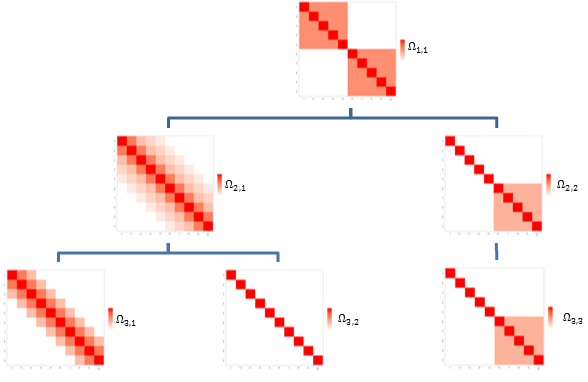
\includegraphics[scale=.7]{graph.png}
\end{center}
\caption{Structure of ground-true networks with 10 variants.}
\label{fig:structure1}
\end{figure}



\begin{figure}
\begin{center}
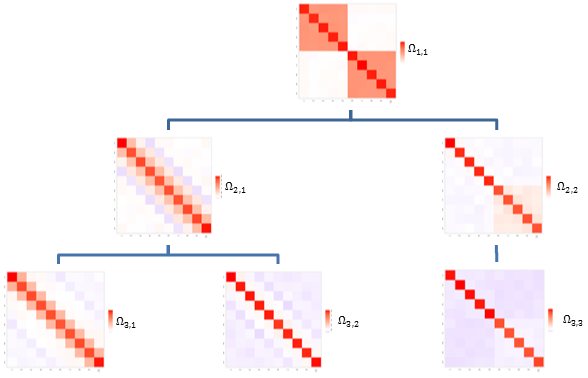
\includegraphics{graphhat100.png}
\end{center}
\caption{Averaged estimation of networks using 50 samples over 100 simulated data with 10 variants.}
\label{fig:structur2}
\end{figure}

\begin{figure}
\begin{center}
 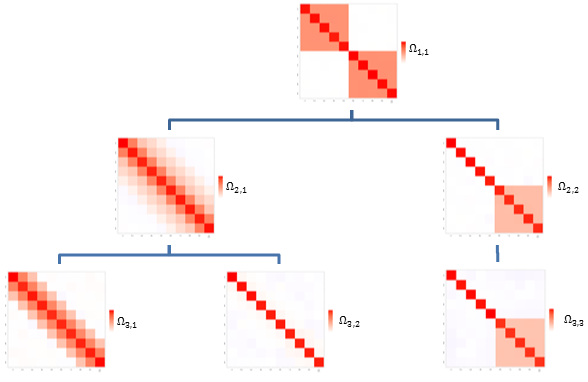
\includegraphics{graphhat1000.png}
\end{center}
\caption{Averaged estimation of networks using 500 samples over 100 simulated data with 10 variants.}
\label{fig:structure3}
\end{figure}

\begin{figure}
\begin{center}
% \includegraphics{av-h-n300.png}
\end{center}
%\caption{STAGEWISE: Averaged estimated networks with 300 samples}
\label{fig:structure4}
\end{figure}

\begin{figure}
\begin{center}
% \includegraphics{n300fused.png}
\end{center}
%\caption{FUSED: Averaged estimated networks with 300 samples}
\label{fig:structure5}
\end{figure}


\begin{figure}
\begin{center}
% \includegraphics{av-h-n100.png}
\end{center}
%\caption{STAGEWISE: Averaged estimated networks with 100 samples}
\label{fig:structure6}
\end{figure}

\begin{figure}
\begin{center}
% \includegraphics{n100fused.png}
\end{center}
%\caption{FUSED: Averaged estimated networks with 100 samples}
\label{fig:structure7}
\end{figure}



\begin{figure}
\begin{center}
 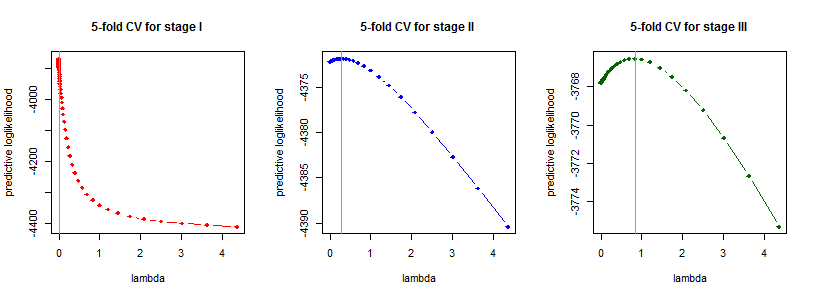
\includegraphics[scale=.6]{lmd-cv.png}
\end{center}
\caption{Cross validated predictive log-likelihood values varying by lambda for n=2000.}
\label{fig:lambda}
\end{figure}
\begin{figure}
\begin{center}
 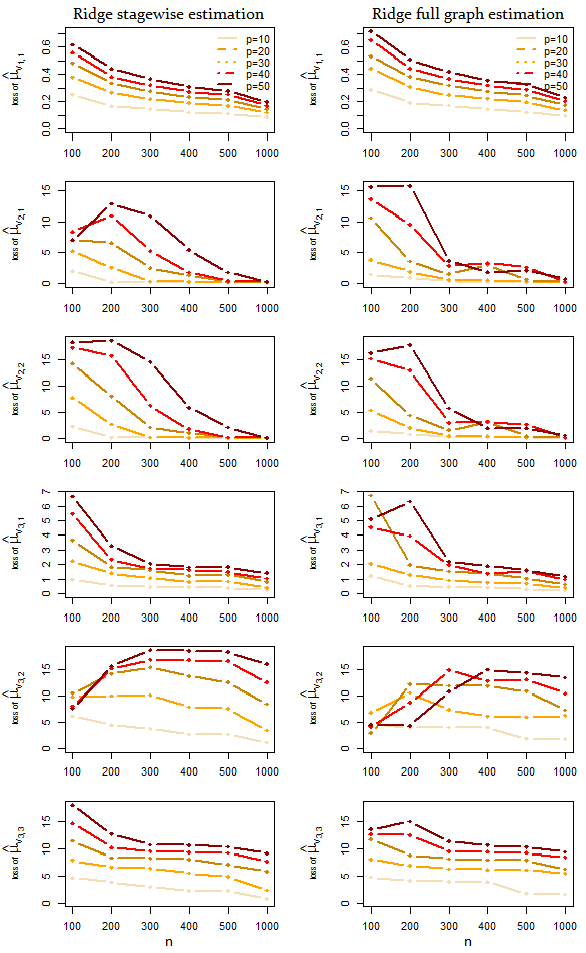
\includegraphics[scale=.6]{mu_err.png}
\end{center}
\caption{Frobenius loss for estimation of mixture means averaged over 50 synthetic data using stagewise and full graph methods with known number of mixture components. First row corresponds to the first stage data, second and third rows correspond to the second stage mixture means, and the rest correspond to the third stage mixture means.}
\label{fig:mu_err}
\end{figure}

\begin{figure}
\begin{center}
 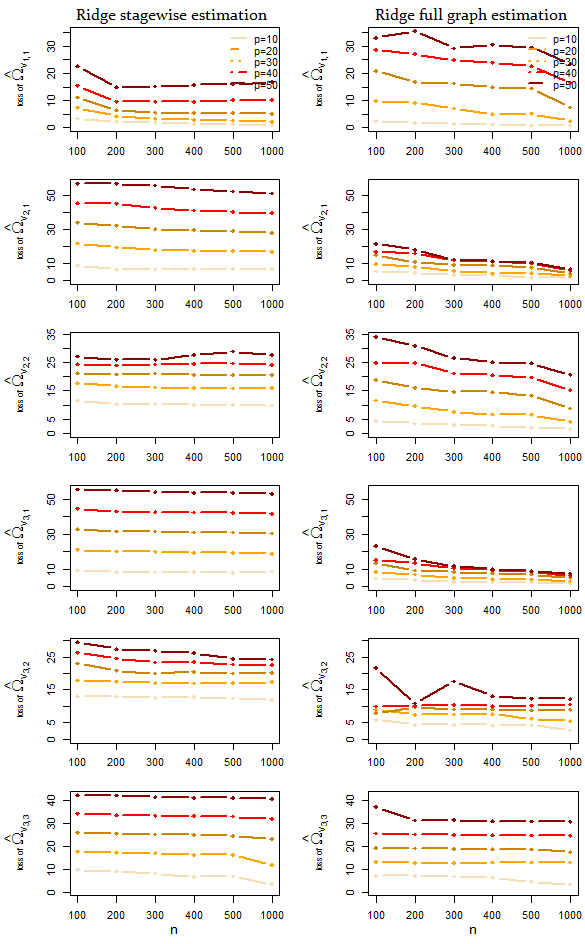
\includegraphics[scale=.6]{thet_err.png}
\end{center}
\caption{Frobenius loss for estimation of mixture precision matrices (i.e. networks) averaged over 50 synthetic data using stagewise and full graph methods with known number of mixture components. First row corresponds to the first stage data network, second and third rows correspond to the second stage networks, and the rest rows correspond to the third stage mixture networks.}
\label{fig:thet_err}
\end{figure}

\begin{figure}
\begin{center}
 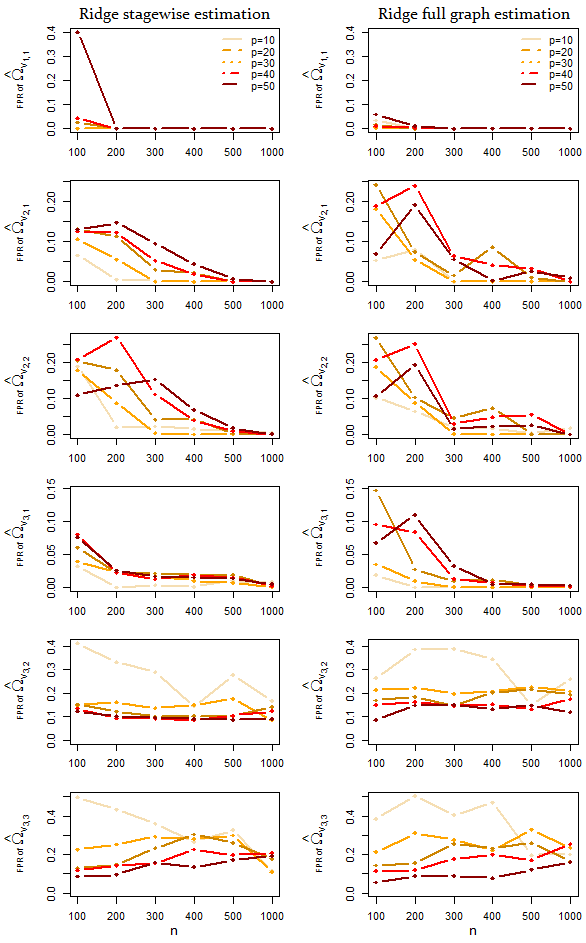
\includegraphics[scale=.6]{FPR.png}
\end{center}
\caption{False positive rate values for sparsified mixture precision matrices (i.e. networks) averaged over 50 synthetic data using stagewise and full graph methods with known number of mixture components. First row corresponds to the first stage data network, second and third rows correspond to the second stage networks, and the rest rows correspond to the third stage mixture networks.}
\label{fig:FPR}
\end{figure}

\begin{figure}
\begin{center}
 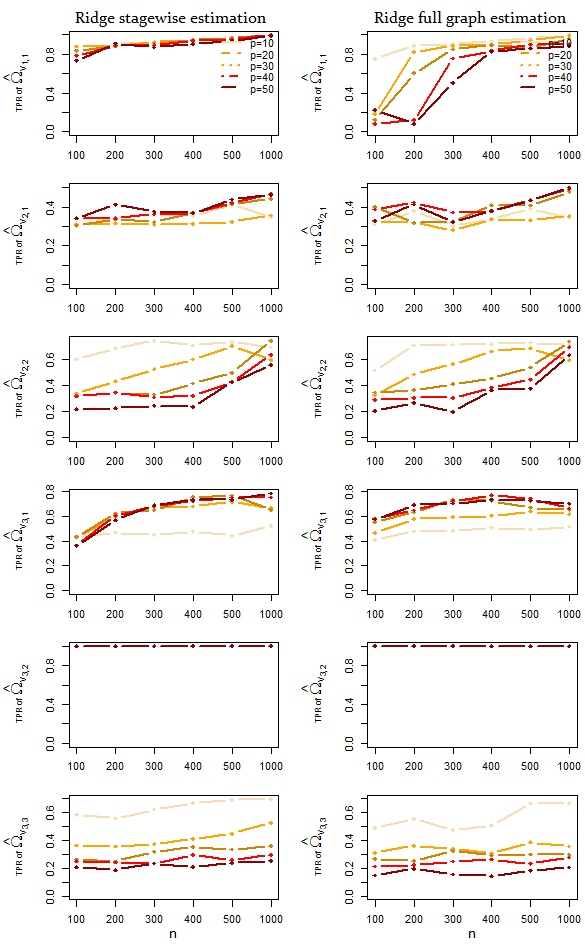
\includegraphics[scale=.6]{TPR.png}
\end{center}
\caption{True positive rate values for sparsified mixture precision matrices (i.e. networks) averaged over 50 synthetic data using stagewise and full graph methods with known number of mixture components. First row corresponds to the first stage data network, second and third rows correspond to the second stage networks, and the rest rows correspond to the third stage mixture networks.}
\label{fig:TPR}
\end{figure}


\begin{figure}
\begin{center}
 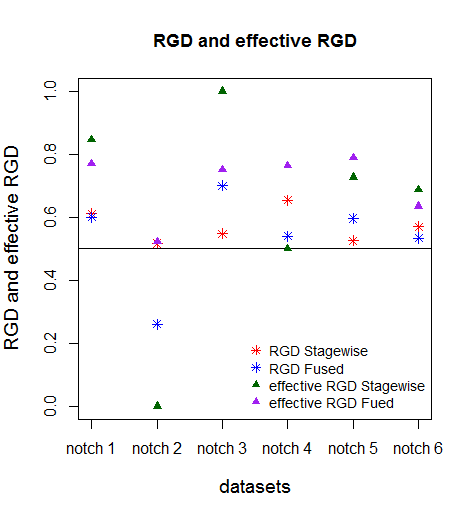
\includegraphics[width=70mm]{RGD.png}
\end{center}
\caption{RGD and eRDG values calculated on the six data from Notch pathway.}
\label{fig:RGD}
\end{figure}


\begin{figure}
\begin{center}
 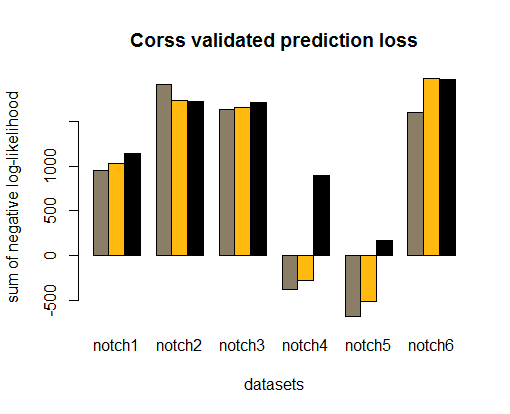
\includegraphics[width=120mm]{pll.png}
\end{center}
\caption{Penalized log-likelihood loss for mixture model with two componenets estimated by stagewise and full graph mixtures, and a related non-mixture model with ridge penalties.}
\label{fig:pll}
\end{figure}

\newpage
\begin{sidewaysfigure}
\begin{center}
 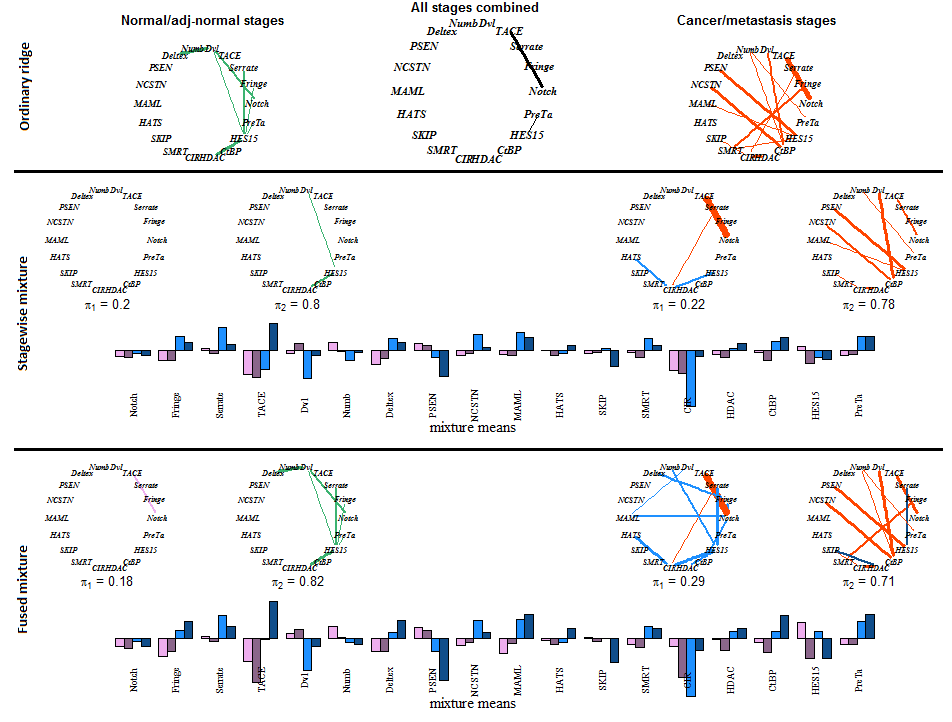
\includegraphics[scale=.8]{notch1.png}
\end{center}
\caption{ Data Notch 1:  Inferred gene complex networks: a) non-mixture ridge, b) stagewise mixture, and d) full graph estimation methods. Estimation of stage-specific component means: c) using stagewise and e) full graoh methods. Intersecting edges of mixture networks are shown by the same color as their correspondent non-mixture networks~(green for the cancer stage and orange for the normal stage).}
\label{fig:notch1}
\end{sidewaysfigure}

\newpage
\begin{sidewaysfigure}
\begin{center}
 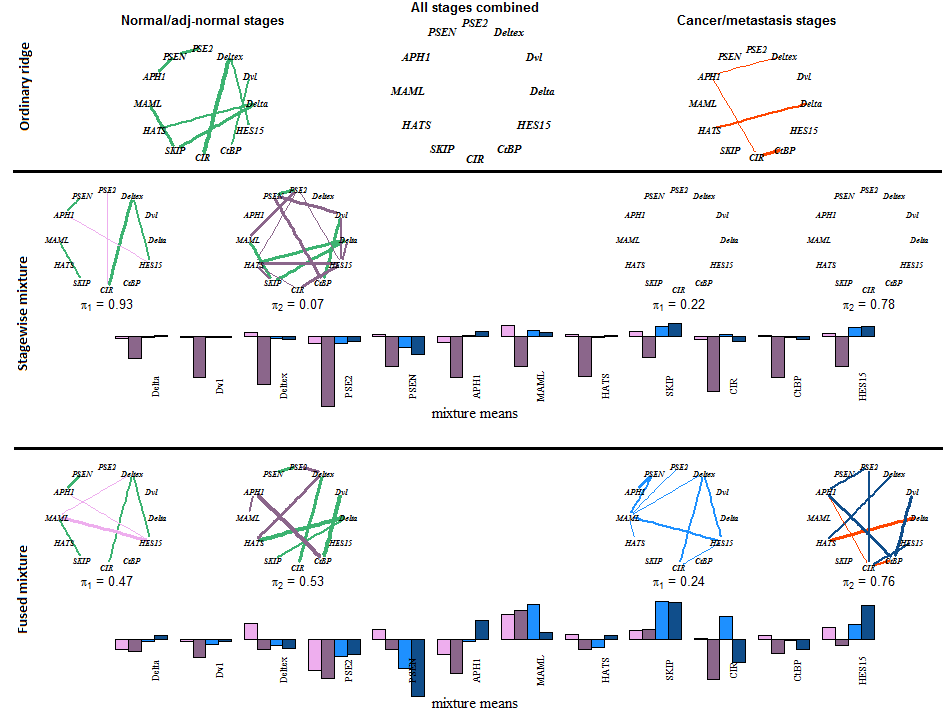
\includegraphics[scale=.8]{notch2.png}
\end{center}
\caption{ Data Notch 2}
\label{fig:notch2}
\end{sidewaysfigure}

\newpage
\begin{sidewaysfigure}
\begin{center}
 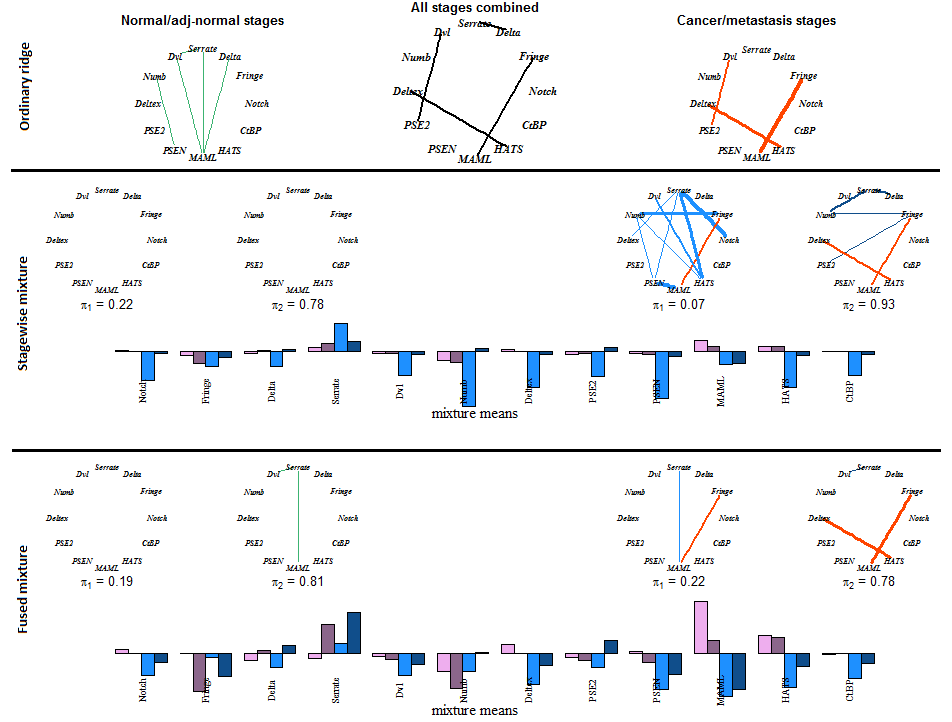
\includegraphics[scale=.8]{notch3.png}
\end{center}
\caption{ Data Notch 3}
\label{fig:notch3}
\end{sidewaysfigure}


\begin{sidewaysfigure}
\begin{center}
 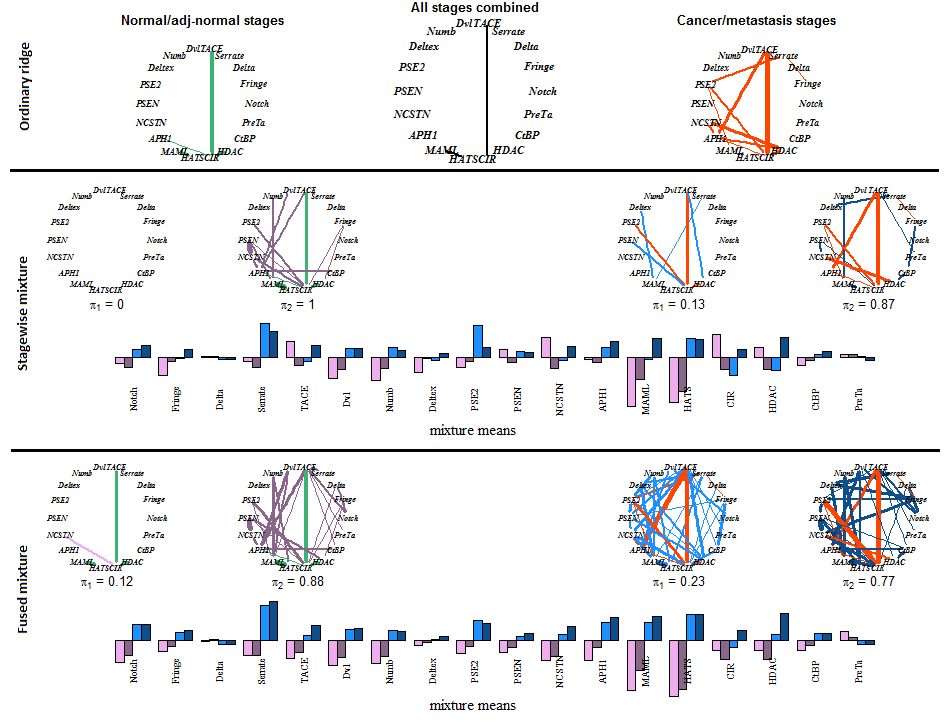
\includegraphics[scale=.8]{notch4.png}
\end{center}
\caption{ Data Notch 4}
\label{fig:notch4}
\end{sidewaysfigure}






\begin{sidewaysfigure}
\begin{center}
 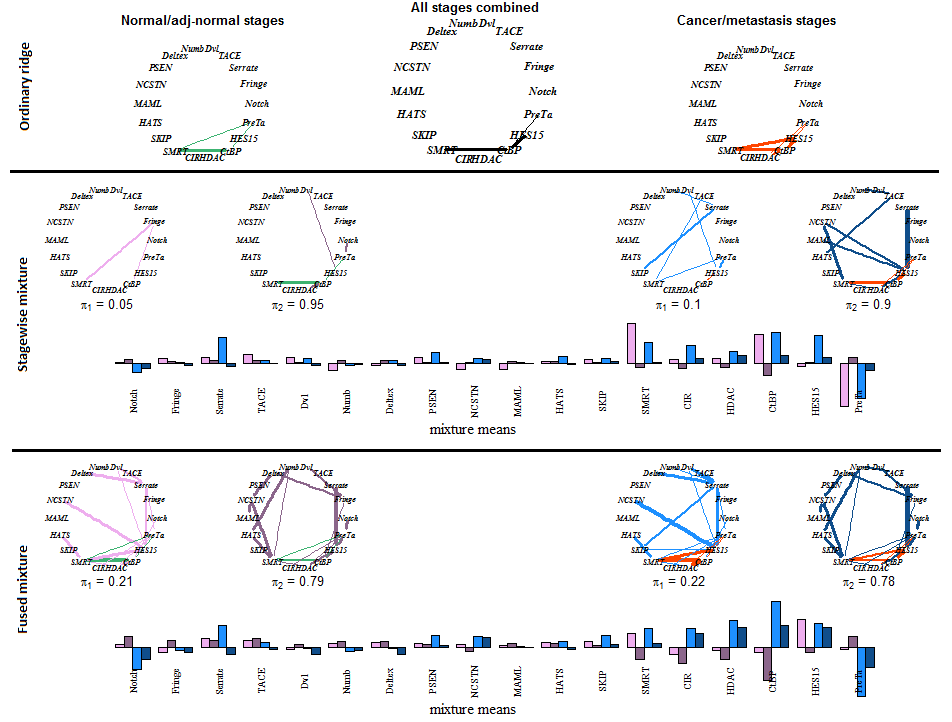
\includegraphics[scale=.8]{notch5.png}
\end{center}
\caption{ \small Data Notch 5}
\label{fig:notch5}
\end{sidewaysfigure}






\newpage
\begin{sidewaysfigure}
\begin{center}
 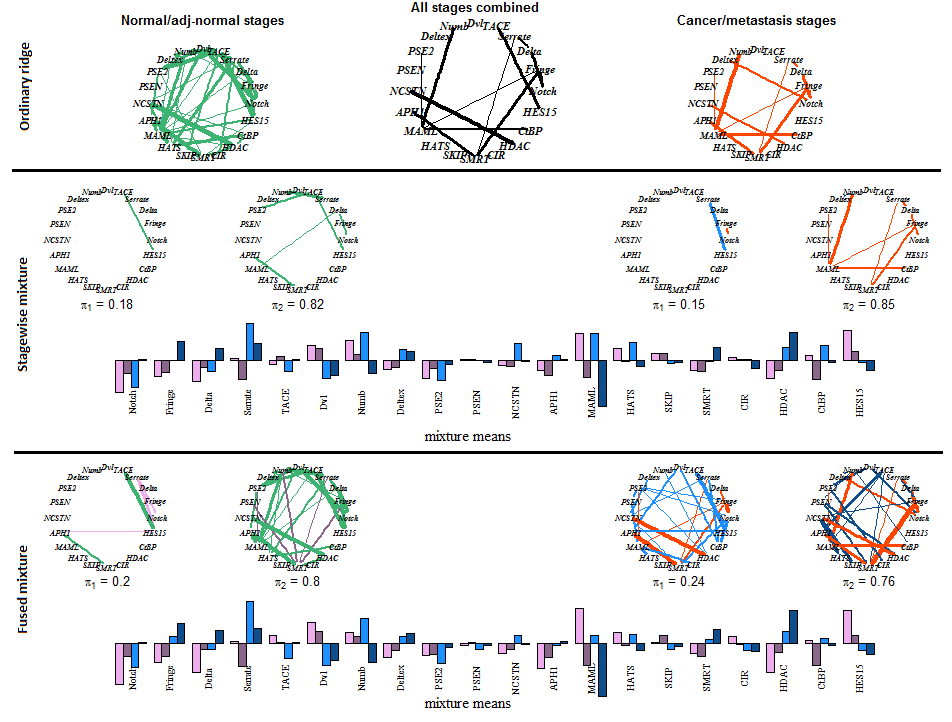
\includegraphics[scale=.8]{notch6.png}
\end{center}
\caption{ Data Notch 6}
\label{fig:notch6}
\end{sidewaysfigure}

\newpage

% Please add the following required packages to your document preamble:
% \usepackage{multirow}
\begin{sidewaystable}
\centering
\caption{Important protein complexes and protein interactions that explain the topological changes from normal stage graphs to those of cancer stage.}
\label{tab:summary}
\begin{tabular}{|llcccccc|}
\hline
\textit{\textbf{Attributes}}                                 & \textit{\textbf{Methods}}                        & \multicolumn{6}{c|}{\textit{\textbf{Data sets}}}                                                                                                                                                                                                                                                                                                                                                                                                                                                                                                                             \\ \hline
\textit{\textbf{}}                                           & \textit{\textbf{}}                               & \textit{\textbf{Notch 1}}                                                                           & \textit{\textbf{Notch 2}}            & \textit{\textbf{Notch 3}}                                                                          & \textit{\textbf{Notch 4}}                                                                             & \textit{\textbf{Notch 5}}                                                                                           & \textit{\textbf{Notch 6}}                                                                    \\ \hline
\multicolumn{1}{|l|}{\textit{\textbf{Hub nodes}}}            & \multicolumn{1}{l|}{\textit{\textbf{Stagewise}}} & \multicolumn{1}{c|}{\begin{tabular}[c]{@{}c@{}}CIR,HES15,\\ CtBP\end{tabular}}                      & \multicolumn{1}{c|}{--}              & \multicolumn{1}{c|}{\begin{tabular}[c]{@{}c@{}}Serrate,HATS,\\ Numb, Fringe,\\  PSEN\end{tabular}} & \multicolumn{1}{c|}{\begin{tabular}[c]{@{}c@{}}TACE,HDAC,\\ MAML,Serrate\end{tabular}}                & \multicolumn{1}{c|}{\begin{tabular}[c]{@{}c@{}}HES15,SMRT,\\ HDAC,PreTa ,\\ Serrate,TACE\end{tabular}}              & \begin{tabular}[c]{@{}c@{}}MAML,Fringe,\\ Serrate\end{tabular}                               \\ \cline{2-8}
\multicolumn{1}{|l|}{\textit{\textbf{}}}                     & \multicolumn{1}{l|}{\textit{\textbf{Fused}}}     & \multicolumn{1}{c|}{\begin{tabular}[c]{@{}c@{}}CIR,CtBP,\\ HES15,Notch,\\ Fringe,Numb\end{tabular}} & \multicolumn{1}{c|}{CIR}             & \multicolumn{1}{c|}{--}                                                                            & \multicolumn{1}{c|}{\begin{tabular}[c]{@{}c@{}}PSE2,TACE,\\ CIRFringe,HDAC,\\ MAML,PSEN\end{tabular}} & \multicolumn{1}{c|}{\begin{tabular}[c]{@{}c@{}}HES15,Serrate,\\ SMRT,CtBP,\\ HDAC,NCSTN,\\ PreTa,Numb\end{tabular}} & \begin{tabular}[c]{@{}c@{}}MAML,NCSTN,\\ SMRT,Notch,\\ PSE2,CtBP,\\ Fringe,PSEN\end{tabular} \\ \hline
\multicolumn{1}{|l|}{\textit{\textbf{Edges with}}}           & \multicolumn{1}{l|}{\textit{\textbf{Stagewise}}} & \multicolumn{1}{c|}{Notch--TACE}                                                                 & \multicolumn{1}{c|}{--}              & \multicolumn{1}{c|}{Notch--Serrate}                                                               & \multicolumn{1}{c|}{Fringe--Serrate}                                                               & \multicolumn{1}{c|}{SMRT--CtBP}                                                                                  & Serrate SMRT                                                                             \\ \cline{3-8}
\multicolumn{1}{|l|}{\textit{\textbf{stronger weights}}}     & \multicolumn{1}{l|}{\textit{\textbf{}}}          & \multicolumn{1}{c|}{PSEN--HES15}                                                                 & \multicolumn{1}{c|}{--}              & \multicolumn{1}{c|}{Fringe--Numb}                                                               & \multicolumn{1}{c|}{PSE2--MAML}                                                                    & \multicolumn{1}{c|}{Serrate HES15}                                                                              & Numb--MAML                                                                                \\ \cline{2-8}
\multicolumn{1}{|l|}{\textit{\textbf{in cancer/metastasis}}} & \multicolumn{1}{l|}{\textit{\textbf{Fused}}}     & \multicolumn{1}{c|}{Notch--TACE}                                                                 & \multicolumn{1}{c|}{CIR--HES15}   & \multicolumn{1}{c|}{Fringe--MAML}                                                               & \multicolumn{1}{c|}{Fringe--Serrate}                                                               & \multicolumn{1}{c|}{SMRT--CtBP}                                                                                  & MAML--CtBP                                                                                \\ \cline{3-8}
\multicolumn{1}{|l|}{\textit{\textbf{stage}}}                & \multicolumn{1}{l|}{\textit{\textbf{}}}          & \multicolumn{1}{c|}{Numb--PreTa}                                                                 & \multicolumn{1}{c|}{PSE2--APH1}   & \multicolumn{1}{c|}{Deltex--HATS}                                                               & \multicolumn{1}{c|}{PSE2--MAML}                                                                    & \multicolumn{1}{c|}{SMRT--HES15}                                                                                 & NCSTN--SKIP                                                                                \\ \hline
\multicolumn{1}{|l|}{\textit{\textbf{Edges with}}}           & \multicolumn{1}{l|}{\textit{\textbf{Stagewise}}} & \multicolumn{1}{c|}{HDAC HES15}                                                                 & \multicolumn{1}{c|}{Deltex CIR}  & \multicolumn{1}{c|}{--}                                                                            & \multicolumn{1}{c|}{CIR--HDAC}                                                                     & \multicolumn{1}{c|}{HDAC--CtBP}                                                                                  & TACE--HES15                                                                               \\ \cline{3-8}
\multicolumn{1}{|l|}{\textit{\textbf{stronger weights}}}     & \multicolumn{1}{l|}{\textit{\textbf{}}}          & \multicolumn{1}{c|}{Dvl--HES15}                                                                  & \multicolumn{1}{c|}{MAML--SKIP}    & \multicolumn{1}{c|}{--}                                                                            & \multicolumn{1}{c|}{PSEN--NCSTN}                                                                   & \multicolumn{1}{c|}{Notch--PreTa}                                                                                & Serrate Numb                                                                             \\ \cline{2-8}
\multicolumn{1}{|l|}{\textit{\textbf{in normal/adjnorm}}}    & \multicolumn{1}{l|}{\textit{\textbf{Fused}}}     & \multicolumn{1}{c|}{Dvl--HES15}                                                                  & \multicolumn{1}{c|}{Deltex--CIR}  & \multicolumn{1}{c|}{Serrate--MAML}                                                              & \multicolumn{1}{c|}{CIR--HDAC}                                                                     & \multicolumn{1}{c|}{SMRT--PreTa}                                                                                 & TACE--HES15                                                                               \\ \cline{3-8}
\multicolumn{1}{|l|}{\textit{\textbf{stage}}}                & \multicolumn{1}{l|}{\textit{\textbf{}}}          & \multicolumn{1}{c|}{Fringe--HES15}                                                               & \multicolumn{1}{c|}{Deltex--PSE2} & \multicolumn{1}{c|}{--}                                                                            & \multicolumn{1}{c|}{Fringe--HDAC}                                                                  & \multicolumn{1}{c|}{Fringe--CtBP}                                                                                & APH1--MAML                                                                                \\ \hline
\multicolumn{1}{|l|}{\textit{\textbf{Edges with}}}           & \multicolumn{1}{l|}{\textit{\textbf{Stagewise}}} & \multicolumn{1}{c|}{--}                                                                             & \multicolumn{1}{c|}{--}              & \multicolumn{1}{c|}{--}                                                                            & \multicolumn{1}{c|}{PSEN--CIR}                                                                     & \multicolumn{1}{c|}{--}                                                                                             & APH1--HES15                                                                               \\ \cline{2-8}
\multicolumn{1}{|l|}{\textit{\textbf{changed sign}}}                 & \multicolumn{1}{l|}{\textit{\textbf{Fused}}}     & \multicolumn{1}{c|}{--}                                                                             & \multicolumn{1}{c|}{--}              & \multicolumn{1}{c|}{--}                                                                            & \multicolumn{1}{c|}{--}                                                                               & \multicolumn{1}{c|}{--}                                                                                             & Numb--Deltex                                                                              \\ \hline
\end{tabular}
\end{sidewaystable}


\end{document}




